\documentclass[a4paper,12pt,twoside]{memoir}

% Castellano
\usepackage[spanish,es-tabla]{babel}
\selectlanguage{spanish}
\usepackage[utf8]{inputenc}
\usepackage[T1]{fontenc}
\usepackage{lmodern} % scalable font
\usepackage{microtype}
\usepackage{placeins}

\RequirePackage{booktabs}
\RequirePackage[table]{xcolor}
\RequirePackage{xtab}
\RequirePackage{multirow}

% Links
\PassOptionsToPackage{hyphens}{url}\usepackage[colorlinks]{hyperref}
\hypersetup{
	allcolors = {red}
}

% Ecuaciones
\usepackage{amsmath}

% Rutas de fichero / paquete
\newcommand{\ruta}[1]{{\sffamily #1}}

% Párrafos
\nonzeroparskip

% Huérfanas y viudas
\widowpenalty100000
\clubpenalty100000

% Evitar solapes en el header
\nouppercaseheads

% Imagenes
\usepackage{graphicx}
\newcommand{\imagen}[2]{
	\begin{figure}[!h]
		\centering
		\includegraphics[width=0.9\textwidth]{#1}
		\caption{#2}\label{fig:#1}
	\end{figure}
	\FloatBarrier
}

\newcommand{\imagenflotante}[2]{
	\begin{figure}%[!h]
		\centering
		\includegraphics[width=0.9\textwidth]{#1}
		\caption{#2}\label{fig:#1}
	\end{figure}
}



% El comando \figura nos permite insertar figuras comodamente, y utilizando
% siempre el mismo formato. Los parametros son:
% 1 -> Porcentaje del ancho de página que ocupará la figura (de 0 a 1)
% 2 --> Fichero de la imagen
% 3 --> Texto a pie de imagen
% 4 --> Etiqueta (label) para referencias
% 5 --> Opciones que queramos pasarle al \includegraphics
% 6 --> Opciones de posicionamiento a pasarle a \begin{figure}
\newcommand{\figuraConPosicion}[6]{%
  \setlength{\anchoFloat}{#1\textwidth}%
  \addtolength{\anchoFloat}{-4\fboxsep}%
  \setlength{\anchoFigura}{\anchoFloat}%
  \begin{figure}[#6]
    \begin{center}%
      \Ovalbox{%
        \begin{minipage}{\anchoFloat}%
          \begin{center}%
            \includegraphics[width=\anchoFigura,#5]{#2}%
            \caption{#3}%
            \label{#4}%
          \end{center}%
        \end{minipage}
      }%
    \end{center}%
  \end{figure}%
}

%
% Comando para incluir imágenes en formato apaisado (sin marco).
\newcommand{\figuraApaisadaSinMarco}[5]{%
  \begin{figure}%
    \begin{center}%
    \includegraphics[angle=90,height=#1\textheight,#5]{#2}%
    \caption{#3}%
    \label{#4}%
    \end{center}%
  \end{figure}%
}
% Para las tablas
\newcommand{\otoprule}{\midrule [\heavyrulewidth]}
%
% Nuevo comando para tablas pequeñas (menos de una página).
\newcommand{\tablaSmall}[5]{%
 \begin{table}
  \begin{center}
   \rowcolors {2}{gray!35}{}
   \begin{tabular}{#2}
    \toprule
    #4
    \otoprule
    #5
    \bottomrule
   \end{tabular}
   \caption{#1}
   \label{tabla:#3}
  \end{center}
 \end{table}
}

%
%Para el float H de tablaSmallSinColores
\usepackage{float}

%
% Nuevo comando para tablas pequeñas (menos de una página).
\newcommand{\tablaSmallSinColores}[5]{%
 \begin{table}[H]
  \begin{center}
   \begin{tabular}{#2}
    \toprule
    #4
    \otoprule
    #5
    \bottomrule
   \end{tabular}
   \caption{#1}
   \label{tabla:#3}
  \end{center}
 \end{table}
}

\newcommand{\tablaApaisadaSmall}[5]{%
\begin{landscape}
  \begin{table}
   \begin{center}
    \rowcolors {2}{gray!35}{}
    \begin{tabular}{#2}
     \toprule
     #4
     \otoprule
     #5
     \bottomrule
    \end{tabular}
    \caption{#1}
    \label{tabla:#3}
   \end{center}
  \end{table}
\end{landscape}
}

%
% Nuevo comando para tablas grandes con cabecera y filas alternas coloreadas en gris.
\newcommand{\tabla}[6]{%
  \begin{center}
    \tablefirsthead{
      \toprule
      #5
      \otoprule
    }
    \tablehead{
      \multicolumn{#3}{l}{\small\sl continúa desde la página anterior}\\
      \toprule
      #5
      \otoprule
    }
    \tabletail{
      \hline
      \multicolumn{#3}{r}{\small\sl continúa en la página siguiente}\\
    }
    \tablelasttail{
      \hline
    }
    \bottomcaption{#1}
    \rowcolors {2}{gray!35}{}
    \begin{xtabular}{#2}
      #6
      \bottomrule
    \end{xtabular}
    \label{tabla:#4}
  \end{center}
}

%
% Nuevo comando para tablas grandes con cabecera.
\newcommand{\tablaSinColores}[6]{%
  \begin{center}
    \tablefirsthead{
      \toprule
      #5
      \otoprule
    }
    \tablehead{
      \multicolumn{#3}{l}{\small\sl continúa desde la página anterior}\\
      \toprule
      #5
      \otoprule
    }
    \tabletail{
      \hline
      \multicolumn{#3}{r}{\small\sl continúa en la página siguiente}\\
    }
    \tablelasttail{
      \hline
    }
    \bottomcaption{#1}
    \begin{xtabular}{#2}
      #6
      \bottomrule
    \end{xtabular}
    \label{tabla:#4}
  \end{center}
}

%
% Nuevo comando para tablas grandes sin cabecera.
\newcommand{\tablaSinCabecera}[5]{%
  \begin{center}
    \tablefirsthead{
      \toprule
    }
    \tablehead{
      \multicolumn{#3}{l}{\small\sl continúa desde la página anterior}\\
      \hline
    }
    \tabletail{
      \hline
      \multicolumn{#3}{r}{\small\sl continúa en la página siguiente}\\
    }
    \tablelasttail{
      \hline
    }
    \bottomcaption{#1}
  \begin{xtabular}{#2}
    #5
   \bottomrule
  \end{xtabular}
  \label{tabla:#4}
  \end{center}
}



\definecolor{cgoLight}{HTML}{EEEEEE}
\definecolor{cgoExtralight}{HTML}{FFFFFF}

%
% Nuevo comando para tablas grandes sin cabecera.
\newcommand{\tablaSinCabeceraConBandas}[5]{%
  \begin{center}
    \tablefirsthead{
      \toprule
    }
    \tablehead{
      \multicolumn{#3}{l}{\small\sl continúa desde la página anterior}\\
      \hline
    }
    \tabletail{
      \hline
      \multicolumn{#3}{r}{\small\sl continúa en la página siguiente}\\
    }
    \tablelasttail{
      \hline
    }
    \bottomcaption{#1}
    \rowcolors[]{1}{cgoExtralight}{cgoLight}

  \begin{xtabular}{#2}
    #5
   \bottomrule
  \end{xtabular}
  \label{tabla:#4}
  \end{center}
}




\graphicspath{ {./img/} }

% Capítulos
\chapterstyle{bianchi}
\newcommand{\capitulo}[2]{
	\setcounter{chapter}{#1}
	\setcounter{section}{0}
	\setcounter{figure}{0}
	\setcounter{table}{0}
	\chapter*{#2}
	\addcontentsline{toc}{chapter}{#2}
	\markboth{#2}{#2}
}

% Apéndices
\renewcommand{\appendixname}{Apéndice}
\renewcommand*\cftappendixname{\appendixname}

\newcommand{\apendice}[1]{
	%\renewcommand{\thechapter}{A}
	\chapter{#1}
}

\renewcommand*\cftappendixname{\appendixname\ }

% Formato de portada
\makeatletter
\usepackage{xcolor}
\newcommand{\tutor}[1]{\def\@tutor{#1}}
\newcommand{\course}[1]{\def\@course{#1}}
\definecolor{cpardoBox}{HTML}{E6E6FF}
\def\maketitle{
  \null
  \thispagestyle{empty}
  % Cabecera ----------------
\noindent
\includegraphics[width=\textwidth]{cabecera}\vspace{1cm}%
  \vfill
  % Título proyecto y escudo informática ----------------
  \colorbox{cpardoBox}{%
    \begin{minipage}{.8\textwidth}
      \vspace{.5cm}\Large
      \begin{center}
      \textbf{TFG del Grado en Ingeniería Informática}\vspace{.6cm}\\
      \textbf{\LARGE\@title{}}
      \end{center}
      \vspace{.2cm}
    \end{minipage}

  }%
  \hfill\begin{minipage}{.20\textwidth}
    
\includegraphics[width=\textwidth]{escudoInfor}
  \end{minipage}
  \vfill
  % Datos de alumno, curso y tutores ------------------
  \begin{center}%
  {%
    \noindent\LARGE
    Presentado por \@author{}\\ 
    en Universidad de Burgos --- \@date{}\\
    Tutor/es: \@tutor{} / César Represa Pérez\\
  }%
  \end{center}%
  \null
  \cleardoublepage
  }
\makeatother


% Datos de portada
\title{PrimeBot \\Documentación Técnica}
\author{Mario Alonso Pulgar}
\tutor{Jesús Enrique Sierra García}
\date{\today}

\begin{document}

\maketitle



\cleardoublepage



%%%%%%%%%%%%%%%%%%%%%%%%%%%%%%%%%%%%%%%%%%%%%%%%%%%%%%%%%%%%%%%%%%%%%%%%%%%%%%%%%%%%%%%%



\frontmatter


\clearpage

% Indices
\tableofcontents

\clearpage

\listoffigures

\clearpage

\listoftables

\clearpage

\mainmatter

\appendix

\apendice{Plan de Proyecto Software}

\section{Introducción}
La planificación de un proyecto es un punto básico para estudiar su viabilidad. En esta fase se estima el trabajo, tiempo y dinero que supondrá llevar a cabo el proyecto.
Hay que definir minuciosamente las fases y las partes del proyecto para obtener unos datos precisos.

La fase de planificación se puede dividir en:

\begin{itemize}
\tightlist
\item
  \textbf{Planificación temporal} 
\item
  \textbf{Estudio de viabilidad} 

\end{itemize}

En la planificación temporal se elabora un calendario donde se estima el tiempo para la realización de cada una de las partes del proyecto.
Se establecerá una fecha de comienzo y una de finalización estimada.

La segunda parte se centra en la viabilidad del proyecto teniendo en cuenta dos aspectos:

\begin{itemize}
\tightlist
\item
  \textbf{Viabilidad económica:} se estiman los costes y beneficios que puede suponer la realización del proyecto.
\item
  \textbf{Viabilidad legal:} Se analizan las leyes y licencias que pueden afectar al desarrollo del proyecto.

\end{itemize}

\section{Planificación temporal}

Al comenzar la planificación del proyecto se decidió utilizar la metodología ágil SCRUM para la gestión del proyecto.~\cite{scrumGuide}
No se ha seguido esta metodología al completo ya que el equipo estaba formado solo por mí y no por un grupo de personas, aunque en líneas generales sí que se ha seguido la filosofía.

\begin{itemize}
\tightlist
\item
  Estrategia de desarrollo incremental a través de sprints y revisiones.
\item
  Duración media de los sprints de 2 semanas.
\item
  Al final de cada sprint se hacía la subida de la parte de código correspondiente.
  \item
  Para cada sprint había una lista de tareas a realizar.
  \item
  Se realizaba una estimación del tiempo que iba a llevar a cabo cada tarea.
\end{itemize}

Para realizar el seguimiento de los sprints y las tareas del proyecto se ha utilizado la plataforma online YouTrack ~\cite{youtrack}, que permite en un panel canvas organizar las tareas, los sprints, la duración de cada sprint e incluso realizar un Diagrama de Gantt con todas las tareas a realizar en el proyecto.

\subsection {Sprint 0 (08/01/2024 - 14/01/2024)}

Para llevar a cabo este sprint se realizó una reunión inicial con el tutor Jesús Enrique Sierra García para comenzar con el proyecto.

En esta reunión se trataron los diferentes objetivos para el proyecto.
Se trataron temas como planificación que se iba a llevar a cabo, metodología ágil a utilizar, características del proyecto y establecer las diferentes herramientas que se iban a utilizar.

Se estimaron 10 horas de trabajo y se invirtieron finalmente 7,5 horas completando todas las tareas.

 \subsection {Sprint 1 (16/01/2024 - 16/02/2024)}
Los objetivos de este sprint eran: configurar y encargar la fabricación de la PCB, seleccionar los componentes que iba a utilizar PrimeBot y seleccionar las pruebas que se van a realizar con esta versión de PrimeBot.

Se estimaron 100 horas de trabajo y se invirtieron finalmente 90 horas completando todas las tareas.
 
 \subsection {Sprint 2 (17/02/2024 - 17/03/2024)}
 
El principal objetivo de este sprint era realizar todo el montaje y todas las pruebas necesarias para asegurar que el funcionamiento de las conexiones y componentes de PrimeBot era el correcto.

Las tareas en las que se dividió este sprint fueron:
 \begin{itemize}
\tightlist
\item
  Montar los componentes de PrimeBot.
\item
  Realizar el Script de Prueba de motores.
\item
  Realizar el Script de Prueba de encoders magnéticos.
  \item
  Realizar el Script de Prueba del selector de posición.
  \item
  Realizar el Script de Prueba de conectividad bluetooth.
    \item
  Realizar el Script de Prueba de los sensores de Distancia.
    \item
  Realizar el Script de Prueba de los sensores de línea.
\end{itemize}

Se estimaron 100 horas de trabajo y se invirtieron finalmente 80 horas completando todas las tareas
 
 \subsection {Sprint 3 (18/03/2024 - 08/04/2024)}
 
 El objetivo de este sprint era realizar el desarrollo del programa que iba a llevar PrimeBot para la prueba de siguelíneas.
 
 Las tareas en las que se dividió este sprint fueron:
 \begin{itemize}
\tightlist
\item
  Implementación de un algoritmo PID ~\cite{ogata2010}sencillo.
\item
  Implementar la conectividad Bluetooth y los parámetros configurables dentro del PID.
\item
  Implementar un algoritmo PID con más parámetros que el inicial.
  \item
  Realizar la optimización del algoritmo PID para obtener el máximo rendimiento posible.
\end{itemize}

Se estimaron 80 horas de trabajo y se invirtieron 90 completando todas las tareas
 
 \subsection {Sprint 4 (09/04/2024 - 02/05/2024)}
  El objetivo de este sprint era realizar el desarrollo del programa que iba a llevar PrimeBot para la prueba de la resolución de cuadrícula.
  
   Las tareas en las que se dividió este sprint fueron:
 \begin{itemize}
\tightlist
\item
  Conectividad Bluetooth para definir estación de salida y de llegada.
\item
  Implementar la representación gráfica de la cuadrícula.
\item
  Implementar el algoritmo que calcula los movimientos desde el origen al destino.
  \item
  Implementar la detección de cruces.
    \item
  Implementar los giros que se realizan en la cuadrícula.
      \item
  Implementar la gestión de puntos bloqueados y caminos alternativos.
\end{itemize}

Este sprint fue el más problemático y el que más tiempo extra que no estaba planeado obligó a invertir. Se estimaron 100 horas de trabajo y se invirtieron 120 horas quedando por cumplir la gestión de puntos bloqueados y caminos alternativos para completar en el siguiente sprint.
 
 \subsection {Sprint 5 (03/05/2024 - 03/06/2024)}
  El objetivo de este sprint era realizar el desarrollo del programa que iba a llevar PrimeBot para la prueba del laberinto.
  
   \begin{itemize}
\tightlist
\item
  Conectividad Bluetooth para iniciar y parar el robot.
\item
  Implementar la detección de paredes con los sensores de distancia.
\item
  Implementar la detección de huecos con los sensores de distancia.
  \item
  Implementar los giros que se realizan dentro del recorrido.
    \item
  Implementar la detección del final del laberinto
      \item
  Implementar la impresión del recorrido por serial vía Bluetooth.
\end{itemize}

Se estimaron 100 horas de trabajo y se invirtieron 70 horas terminando todas las tareas, pero fue necesario invertir otras 50 horas para completar la tarea faltante del sprint anterior.  
  
   \subsection {Sprint 6 (16/01/2024 - 03/06/2024)}
  El objetivo de este sprint era realizar el desarrollo del la página web que iba a acompañar al proyecto.
  
     \begin{itemize}
\tightlist
\item
  Compra del dominio.
\item
  Creación de HomePage.
\item
  Diseño de Landing Page PrimeBot.
  \item
  Implementar Landing Page PrimeBot.
        \item
  Incluir contenido relacionado con PrimeBot.
    \item
  Incluir vídeos multimedia de PrimeBot funcionando.
\end{itemize}
  Se estimaron 90 horas de trabajo y se invirtieron 70 horas completando todas las tareas.  
  
   \subsection {Sprint 7 (03/06/2024 - 09/06/2024)}
  El objetivo de este sprint era terminar la memoria, los anexos y todo el material relativo a la entrega del proyecto.
\begin{itemize}
\tightlist
\item
  Terminar la memoria en LaTex.
\item
  Terminar los anexos en LaTex.
\item
  Realizar los dos vídeos necesarios para la entrega.
  \item
  Preparar material para el día de la defensa.
\end{itemize}

Se estimaron 40 horas de trabajo y se invirtieron 40 horas completando todas las tareas.

\subsection {Resumen}
Finalmente en el proyecto de PrimeBot se han invertido aproximadamente las mismas horas de trabajo que se había estimado en un inicio pero no con la misma distribución en los sprints, siendo necesarias utiliizar horas de un sprint en el sprint posterior.

En la siguiente tabla se pueden ver las horas que se han invertido en cada parte del desarrollo de PrimeBot:

 \begin{table}[h]
   \rowcolors {2}{gray!35}{}
\begin{tabular}{| r | l |}
\hline
Planificación del proyecto & 27,5 horas \\
\hline
Documentación & 70 horas \\
\hline
Características & 400 horas \\
\hline
Desarrollo web & 70 horas\\
\hline
Diseño de piezas & 50 horas\\
\hline
Optimización de programas & 100 horas \\
\hline
Total & 717,5 horas \\
\hline
\end{tabular}
   \caption{Resumen horas dedicadas a cada apartado de PrimeBot}
   \label{A.1}
 \end{table}

\section{Estudio de viabilidad}

\subsection{Viabilidad económica}
En este apartado se analizarán los costes y los posibles beneficios que se pueden obtener con este proyecto realizándolo en un entorno empresarial real.

\subsubsection{Costes}

Los costes del proyecto se pueden desglosar en varias categorías, vamos a detallar cada una de ellas:
\\
\textbf{Costes de Personal}

El proyecto ha sido llevado a cabo por un equipo de desarrollo web y por un desarrollador empleado a tiempo completo durante cinco meses.

Del desarrollador se considera el siguiente salario:

 \begin{table}[h]
   \rowcolors {2}{gray!35}{}
\begin{tabular}{| r | l |}
\hline
Concepto & Coste \\
\hline
Salario Neto & 1281€ \\
\hline
IRPF & 1507,15€ \\
\hline
Seguridad Social & 642,85€ \\
\hline
Salario Bruto & 2150€ \\
\hline
\end{tabular}
   \caption{Tabla de los costes de personal }
   \label{A.2}
 \end{table}
El total por tanto durante 5 meses en salario bruto será de 10.750€
El coste del desarrollo web se define como un presupuesto cerrado que tiene un coste total de 500€ IVA Incluido y se divide en diseño y desarrollo:

 \begin{table}[h]
   \rowcolors {2}{gray!35}{}
\begin{tabular}{| r | l |}
\hline
Concepto & Coste \\
\hline
Diseño Web & 200€ \\
\hline
Desarrollo & 300€ \\
\hline
\end{tabular}
   \caption{Tabla de los costes desarrollo web}
   \label{A.3}
 \end{table}
 
\textbf{Costes de Hardware}

En este apartado se revisan todos los costes en dispositivos y componentes de Primebot que han sido necesarios para el desarrollo del proyecto.
 \begin{table}[h]
\begin{tabular}{| r | l |}
\hline
Concepto & Coste \\
\hline
Fabricación PCB & 29 € \\
\hline
Arduino Nano ~\cite{arduinoNanoEvery} & 19 € \\
\hline
QTR8A ~\cite{pololuQTR8A} & 12.04 € \\
\hline
OPT3101 ~\cite{pololuOPT3101} & 45.38 € \\
\hline
Bluetooth & 4.54 € \\
\hline
Driver de Motores & 5.99€ \\
\hline
Batería & 4.50 € \\
\hline
Motores N20 & 10.90 € \\
\hline
Encoders Magnéticos & 10.29 € \\
\hline
\end{tabular}
   \caption{Tabla de los costes de hardware}
   \label{A.4}
 \end{table}
 
Por tanto el total de la construcción de PrimeBot a nivel de hardware sería de 141,64 €

\textbf{Costes Varios}

En este apartado se revisan el resto de costes del proyecto.

 \begin{table}[h]
\begin{tabular}{| r | l |}
\hline
Concepto & Coste \\
\hline
Hosting & 6€ / mes \\
\hline
Dominio & 14,90€ / año \\
\hline
\end{tabular}
   \caption{Tabla de costes varios}
   \label{A.5}
 \end{table}
 
En el total de los costes hay que incluir que el hosting de momento se ha mantenido durante 5 meses, además del dominio haría un total de 44,90€.

\textbf{Costes Totales}

A continuación se adjunta una tabla con los costes totales de cada sección de PrimeBot en caso de llevarse a cabo en un entorno industrial.
 \begin{table}[h]
\begin{tabular}{| r | l |}
\hline
Concepto & Coste \\
\hline
Costes de Personal & 10.750€ \\
\hline
Costes desarrollo web & 500€ \\
\hline
Costes mantenimiento web & 44,90€ \\
\hline
Costes hardware & 141,64€ \\
\hline
Total & 11.436,64€ \\
\hline
\end{tabular}
   \caption{Tabla de costes totales}
   \label{A.6}
 \end{table}

\textbf{Ingresos}

PrimeBot es un proyecto sólido y con un gran rendimiento que se podría emplear en numerosas ediciones del ASTI Robotics Challenge para pelear por los primeros premios, además también se podría comercializar en kit para que los equipos que quieran participar adquieran el kit a nivel de hardware y desarrollen sus propios programas.

Se considerará que en 5 años, al menos en uno se consiga el primer premio del ASTI Robotics Challenge y que un kit de Hardware se venderá al doble del precio de coste de los materiales. 
 \begin{table}[h]
\begin{tabular}{| r | l |}
\hline
Concepto & Cantidad \\
\hline
Ganador ASTI Robotics Challenge & 3.000€ \\
\hline
Venta kit educativo & 299€ \\
\hline
\end{tabular}
   \caption{Tabla de ingresos potenciales}
   \label{A.7}
 \end{table}
 
\subsection{Viabilidad legal}

En esta sección se discutirán los temas relacionados con las licencias que puedan estar relacionadas con cualquiera de los ámbitos de este proyecto.

\subsubsection{Software}

Primero hay que elegir cuál sería la licencia más conveniente para el proyecto de PrimeBot.
Hay que elegir que derechos queremos proporcionar a los usuarios y cuáles no.

En mi caso quiero que PrimeBot sea un proyecto de software libre y código abierto por lo que seleccionaré la licencia más permisible posible con los usuarios.

Dentro de las licencias, la más permisible es la licencia MIT.

MIT Permite a los usuarios realizar uso, copia, modificación, fusión, publicación, sublicencia y venta de copias del software.

MIT Es compatible con muchas otras licencias de software libre y de código abierto.

\subsubsection{Documentacion}

Para la documentación he seleccionado utilizar una licencia Creative Commons ya que están enfocadas a licenciar este tipo de contenidos, en concreto he seleccionado Creative Commons Attribution 4.0 International (CC-BY-4.0) que establece lo siguiente:

\subsubsection{Imágenes y vídeos}

En la documentación del proyecto no se han utilizado imágenes de terceros por lo que tanto las imágenes como los vídeos son propias del proyecto y cuentan con la misma licencia que la documentación (CC-BY-4.0)





\apendice{Especificación de Requisitos}

\section{Introducción}

En esta sección se recoge la especificación de requisitos que define el comportamiento del sistema desarrollado.
Esta sección tiene como objetivo documentar correctamente la forma en la que se ha desarrollado PrimeBot.

Se han seguido las recomendaciones del estándar IEEE 830-1998 que manifiesta que una buena especificación de requisitos de software debe ser:

\begin{itemize}
\tightlist
\item
  \textbf{Completa}: todos los requerimientos deben estar reflejados en
  ella y todas las referencias deben estar definidas.
\item
  \textbf{Consistente}: debe ser coherente con los propios
  requerimientos y también con otros documentos de especificación.
\item
  \textbf{Inequívoca}: la redacción debe ser clara de modo que no se
  pueda mal interpretar.
\item
  \textbf{Correcta}: el software debe cumplir con los requisitos de la
  especificación.
\item
  \textbf{Trazable}\emph{: s}e refiere a la posibilidad de verificar la
  historia, ubicación o aplicación de un ítem a través de su
  identificación almacenada y documentada.
\item
  \textbf{Priorizable}: los requisitos deben poder organizarse
  jerárquicamente según su relevancia para el negocio y clasificándolos
  en esenciales, condicionales y opcionales.
\item
  \textbf{Modificable}: aunque todo requerimiento es modificable, se
  refiere a que debe ser fácilmente modificable.
\item
  \textbf{Verificable}: debe existir un método finito sin costo para
  poder probarlo.
\end{itemize}

\section{Objetivos generales}
El proyecto persigue los siguientes objetivos generales:

\begin{itemize}
\tightlist
\item
  Desarrollar una algoritmo PID eficiente y de alto rendimiento para seguir línea negra.
\item
  Implementar un algoritmo para la resolución de la prueba de cuadrícula.
\item
  Implementar un algoritmo eficiente para la resolución de laberintos.
\item
  Establecer protocolos de comunicación Bluetooth a tiempo real para aumentar el rendimiento de PrimeBot.
  \item
  Permitir ejecutar varios programas a la vez sin necesidad de un PC.
\end{itemize}

\section{Catálogo de requisitos}\label{catalogo-de-requisitos}

A continuación, se enumeran los requisitos específicos derivados de los objetivos generales del proyecto.
\subsection{Requisitos funcionales}\label{requisitos-funcionales}

\begin{itemize}
\tightlist
\item
  \textbf{RF-1 Seguimiento de línea:} PrimeBot debe ser capaz de seguir líneas negras sobre un fondo blanco utilizando los sensores QTR8A.
  \begin{itemize}
  \tightlist
  \item
    \textbf{RF-1.1 Detección de Líneas:} Los sensores QTR8A detectan el contraste entre la línea negra y el fondo blanco.
  \item
    \textbf{RF-1.2 Ajuste de Dirección:} El algoritmo PID ajusta la dirección del robot basándose en la información de los sensores.
  \item
    \textbf{RF-1.3 Calibración inicial:} antes de comenzar las pruebas, PrimeBot debe calibrar sus sensores QTR8A para seguir correctamente la línea negra.
\end{itemize}
\item
  \textbf{RF-2 Navegacion en cuadricula :} PrimeBot debe moverse de una estación de origen a una estación de destino en una cuadrícula predefinida.
  \begin{itemize}
  \tightlist
  \item
    \textbf{RF-2.1 Detección de Cruces:} El robot detecta los cruces en la cuadrícula utilizando los sensores QTR8A.
  \item
    \textbf{RF-2.2 Cálculo de Rutas:} El robot calcula la ruta más eficiente desde la estación de origen a la de destino.
  \item
    \textbf{RF-2.3 Evitar puntos bloqueados:} PrimeBot debe ser capaz de calcular rutas alternativas ante puntos de la cuadrícula bloqueados.
  \end{itemize}
\item
  \textbf{RF-3 Resolución de laberintos: } PrimeBot debe navegar y resolver laberintos utilizando algoritmos de búsqueda y sensores OPT3101.
  \begin{itemize}
  \tightlist
  \item
    \textbf{RF-3.1 Detección de Paredes: } Los sensores OPT3101 detectan la presencia de paredes en el laberinto.
  \item
    \textbf{RF-3.2 Detección de huecos: } PrimeBot debe ser capaz de detectar los huecos que hay en el laberinto para navegar sobre él.
  \end{itemize}

\end{itemize}

\subsection{Requisitos no funcionales}\label{requisitos-no-funcionales}
\begin{itemize}
\tightlist
\item
\textbf{RNF-1 Rendimiento:} PrimeBot debe operar con un tiempo de respuesta mínimo y eficiente.
\item
\textbf{RNF-2 Confiabilidad:} PrimeBot debe ser confiable y operar sin fallos durante largos periodos.
\item
\textbf{RNF-3 Usabilidad:} PrimeBot debe ser fácil de usar e interactuar.

\begin{itemize}
\tightlist
\item
\textbf{RNF-3.1 Interfaz de Usuario:} El robot debe ser controlable mediante una interfaz de usuario sencilla y los ajustes vía Bluetooth deben ser intuitivos.
\end{itemize}
\item
\textbf{RNF-4 Mantenibilidad:} El código y hardware de PrimeBot deben ser fáciles de mantener y actualizar.

\begin{itemize}
\tightlist
\item
\textbf{RNF-4.1 Actualización de Software y Hardware:} Las actualizaciones deben poder realizarse sin necesidad de una reestructuración completa.
\end{itemize}
\item
\textbf{RNF-5 Portabilidad:} PrimeBot debe ser portátil y fácil de transportar.

\begin{itemize}
\tightlist
\item
\textbf{RNF-5.1 Peso y Dimensiones:} El robot debe ser ligero y compacto, con un peso inferior a 1 kg y dimensiones manejables.
\end{itemize}
\item
\textbf{RNF-6 Escalabilidad:} PrimeBot debe permitir futuras expansiones y mejoras.

\begin{itemize}
\tightlist
\item
\textbf{RNF-6.1 Adición de Nuevos Componentes:} La arquitectura debe permitir la adición de nuevos sensores y módulos sin necesidad de un rediseño significativo.
\end{itemize}
\item
\textbf{RNF-7 Seguridad:} PrimeBot debe operar de manera segura tanto para los usuarios como para el entorno.
\end{itemize}

\newpage
\section{Diagramas UML}

\subsection{Diagrama de flujo}

A continuación se muestra un diagrama de flujo de la selección de programa de PrimeBot (Figura B.1).
Esta selección se realiza con el selector DIP y el pulsador que hay en la parte trasera del PCB de PrimeBot

\begin{figure}[h]
	\centering
	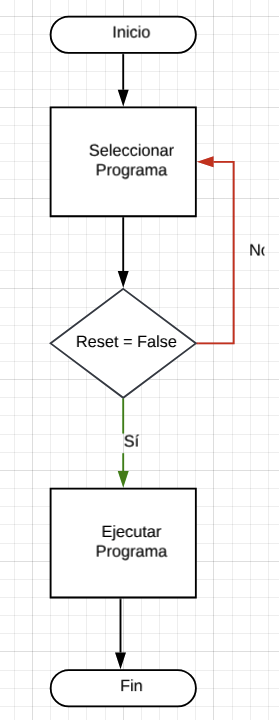
\includegraphics[width=0.25\textwidth]{anexos/diagramaDeFlujo}
	\caption{Diagrama de Flujo.}
	\label{fig:B.1}
\end{figure}
\newpage
\subsection{Diagramas de secuencias}
A continuación se colocan los diagramas de secuencias de las diferentes pruebas que realiza PrimeBot.
\subsubsection{Prueba de siguelineas}
La prueba de siguelíneas se realiza de forma ininterrumpida hasta que se vuelve a pulsar el botón con otro programa seleccionado (Figura B.2).
\begin{figure}[h]
	\centering
	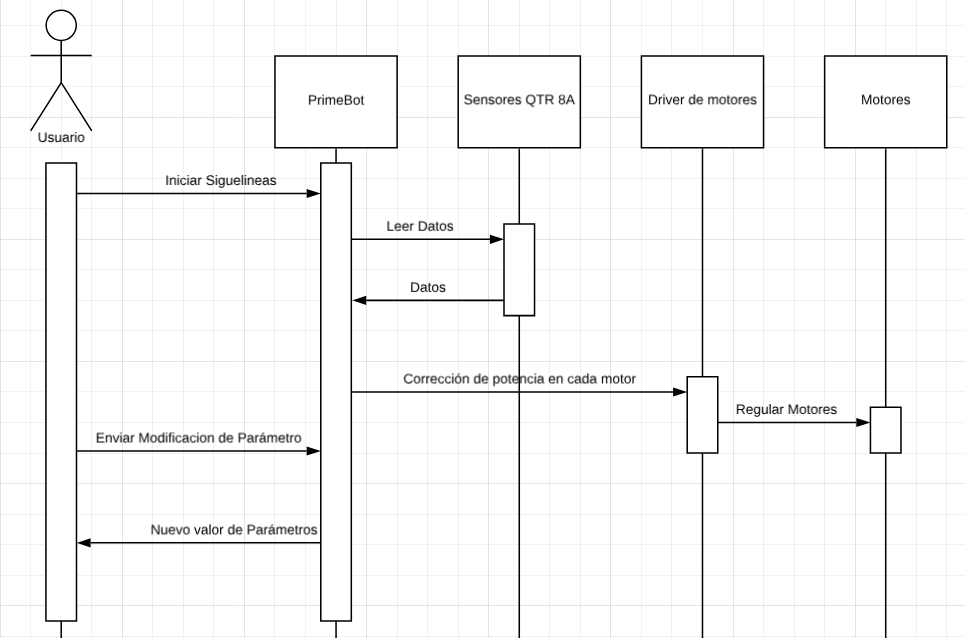
\includegraphics[width=0.5\textwidth]{anexos/diagramaSiguelineas}
	\caption{Diagrama de secuencia programa siguelineas.}
	\label{fig:B.2}
\end{figure}

\subsubsection{Prueba de cuadrícula}

La prueba de la cuadrícula es la más compleja y se realiza a partir de unos argumentos que el usuario aporta a PrimeBot.

En el diagra de secuencias se puede ver la ejecución completa del programa (Figura B.3).

\begin{figure}[h]
	\centering
	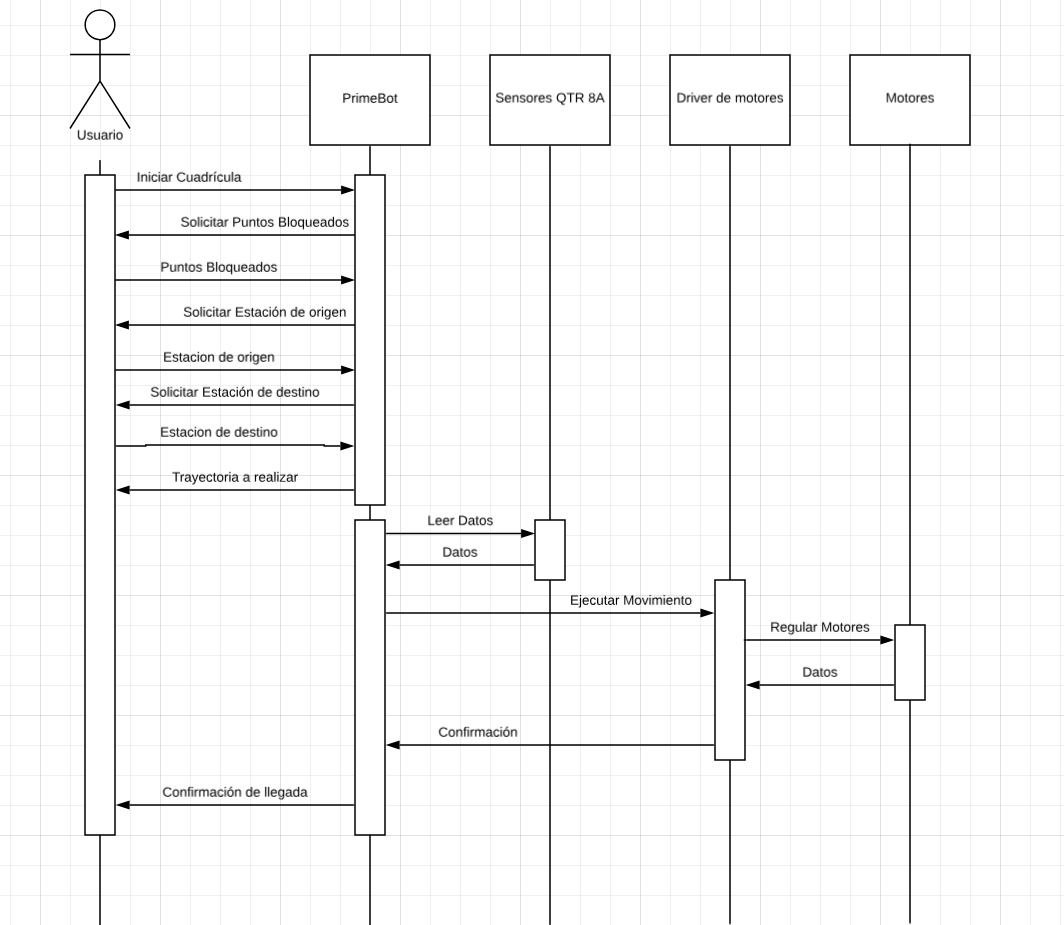
\includegraphics[width=0.5\textwidth]{anexos/diagramaCuadricula}
	\caption{Diagrama de secuencia programa de resolución de cuadrícula.}
	\label{fig:B.3}
\end{figure}
\newpage
\subsubsection{Prueba de laberinto}

\begin{figure}[h]
	\centering
	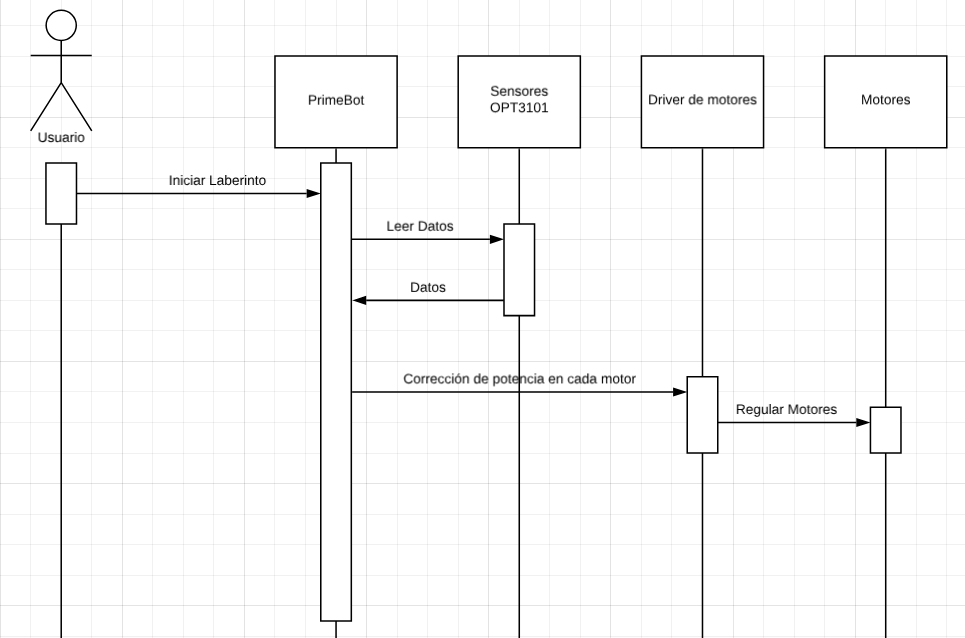
\includegraphics[width=0.5\textwidth]{anexos/diagramaLaberinto}
	\caption{Diagrama de secuencia programa de resolución de laberinto.}
	\label{fig:B.2}
\end{figure}


\newpage
\section{Especificación de requisitos}

En esta sección se desarrollará cada caso de uso del sistema.
\begin{table}[p]
	\centering
	\begin{tabularx}{\linewidth}{ p{0.21\columnwidth} p{0.71\columnwidth} }
		\toprule
		\textbf{CU-1}    & \textbf{Calibración de Sensores}\\
		\toprule
		\textbf{Versión}              & 1.0    \\
		\textbf{Autor}                & Mario Alonso Pulgar \\
		\textbf{Requisitos asociados} & RF-1.3 \\
		\textbf{Descripción}          & PrimeBot calibra sus sensores QTR para una mejor precisión en el seguimiento de líneas.\\
		\textbf{Precondición}         & PrimeBot está encendido y los sensores QTR están conectados.\\
		\textbf{Acciones}             &
		\begin{enumerate}
			\def\labelenumi{\arabic{enumi}.}
			\tightlist
			\item El usuario selecciona la opción de calibración en el dip-switch.
			\item PrimeBot enciende los LEDs de calibración.
			\item PrimeBot calibra los sensores durante 400 iteraciones.
			\item PrimeBot apaga los LEDs de calibración.
		\end{enumerate}\\
		\textbf{Postcondición}        & Los sensores QTR están calibrados y listos para su uso.  \\
		\textbf{Excepciones}          & Si la calibración falla, PrimeBot avisa al usuario y detiene la operación.  \\
		\textbf{Importancia}          & Alta \\
		\bottomrule
	\end{tabularx}
	\caption{CU-1 Calibración de Sensores.}
\end{table}

% Caso de Uso 1 -> Consultar Experimentos.
\begin{table}[p]
	\centering
	\begin{tabularx}{\linewidth}{ p{0.21\columnwidth} p{0.71\columnwidth} }
		\toprule
		\textbf{CU-2}    & \textbf{Seguimiento de linea}\\
		\toprule
		\textbf{Versión}              & 1.0    \\
		\textbf{Autor}                & Mario Alonso Pulgar \\
		\textbf{Requisitos asociados} & RF-1, RF-1.1, RF-1.2\\
		\textbf{Descripción}          & PrimeBot sigue una línea negra sobre un fondo blanco utilizando los sensores QTR8A.\\
		\textbf{Precondición}         & PrimeBot está encendido, los sensores QTR8A están calibrados y está seleccionado el programa 0001\\
		\textbf{Acciones}             &
		\begin{enumerate}
			\def\labelenumi{\arabic{enumi}.}
			\tightlist
				\item El usuario coloca PrimeBot al inicio de una línea negra.
				\item PrimeBot detecta la línea utilizando los sensores QTR8A.
				\item PrimeBot ajusta su dirección mediante el algoritmo PID.
				\item PrimeBot sigue la línea hasta el final del recorrido.
		\end{enumerate}\\
		\textbf{Postcondición}        & PrimeBot sigue la línea negra sin salirse del camino.  \\
		\textbf{Excepciones}          & Si PrimeBot pierde la línea, recalibra los sensores y vuelve a buscar la línea.  \\
		\textbf{Importancia}          & Alta \\
		\bottomrule
	\end{tabularx}
	\caption{CU-2 Seguimiento de Líneas.}
\end{table}

\begin{table}[p]
	\centering
	\begin{tabularx}{\linewidth}{ p{0.21\columnwidth} p{0.71\columnwidth} }
		\toprule
		\textbf{CU-3}    & \textbf{Navegación en Cuadrícula}\\
		\toprule
		\textbf{Versión}              & 1.0    \\
		\textbf{Autor}                & Mario Alonso Pulgar \\
		\textbf{Requisitos asociados} & RF-2, RF-2.1, RF-2.2, RF-2.3 \\
		\textbf{Descripción}          & PrimeBot se mueve de una estación de origen a una estación de destino en una cuadrícula predefinida.\\
		\textbf{Precondición}         & PrimeBot está encendido, los sensores QTR8A están calibrados y está seleccionado el programa 0010\\
		\textbf{Acciones}             &
		\begin{enumerate}
			\def\labelenumi{\arabic{enumi}.}
			\tightlist
				\item El usuario indica las estaciones de origen y destino a través de Bluetooth.
				\item PrimeBot detecta los cruces en la cuadrícula utilizando los sensores QTR8A.
				\item PrimeBot calcula la ruta más eficiente.
				\item PrimeBot se mueve a través de la cuadrícula hasta llegar a la estación de destino.
		\end{enumerate}\\
		\textbf{Postcondición}        & PrimeBot llega a la estación de destino. \\
		\textbf{Excepciones}          & Si PrimeBot pierde la línea, recalibra los sensores y vuelve a buscar la línea.  \\
		\textbf{Importancia}          & Alta \\
		\bottomrule
	\end{tabularx}
	\caption{CU-3 Navegación en Cuadrícula.}
\end{table}

\begin{table}[p]
	\centering
	\begin{tabularx}{\linewidth}{ p{0.21\columnwidth} p{0.71\columnwidth} }
		\toprule
		\textbf{CU-4}    & \textbf{Resolución de Laberintos}\\
		\toprule
		\textbf{Versión}              & 1.0    \\
		\textbf{Autor}                & Mario Alonso Pulgar \\
		\textbf{Requisitos asociados} & RF-3, RF-3.1, RF-3.2 \\
		\textbf{Descripción}          & PrimeBot navega y resuelve laberintos utilizando algoritmos de búsqueda y sensores OPT3101. \\
		\textbf{Precondición}         & PrimeBot está encendido, los sensores OPT3101 están calibrados y está seleccionado el programa 0011\\
		\textbf{Acciones}             &
		\begin{enumerate}
			\def\labelenumi{\arabic{enumi}.}
			\tightlist
				\item El usuario coloca PrimeBot en la entrada del laberinto.
				\item PrimeBot utiliza los sensores OPT3101 para detectar paredes.
				\item PrimeBot emplea un algoritmo de búsqueda para planificar su ruta.
				\item PrimeBot navega a través del laberinto.
				\item PrimeBot llega a la salida del laberinto.
		\end{enumerate}\\
		\textbf{Postcondición}        & PrimeBot encuentra la salida del laberinto.\\
		\textbf{Excepciones}          & Si PrimeBot encuentra un obstáculo inesperado, recalcula la ruta y continúa navegando. \\
		\textbf{Importancia}          & Alta \\
		\bottomrule
	\end{tabularx}
	\caption{CU-4 Resolución de Laberintos}
\end{table}

\begin{table}[p]
	\centering
	\begin{tabularx}{\linewidth}{ p{0.21\columnwidth} p{0.71\columnwidth} }
		\toprule
		\textbf{CU-5}    & \textbf{Ajuste de Parámetros PID}\\
		\toprule
		\textbf{Versión}              & 1.0    \\
		\textbf{Autor}                & Mario Alonso Pulgar \\
		\textbf{Requisitos asociados} & RNF-3 \\
		\textbf{Descripción}          & El usuario ajusta los parámetros del controlador PID para optimizar el rendimiento de PrimeBot.\\
		\textbf{Precondición}         & PrimeBot está encendido y conectado al sistema de control.\\
		\textbf{Acciones}             &
		\begin{enumerate}
			\def\labelenumi{\arabic{enumi}.}
			\tightlist
			\item El usuario selecciona el parámetro PID a ajustar (Kp, Ki, Kd, Kv).
			\item El usuario incrementa o decrementa el valor del parámetro seleccionado.
			\item PrimeBot ajusta su comportamiento en función del nuevo valor del parámetro PID.
		\end{enumerate}\\
		\textbf{Postcondición}        & Los parámetros PID están ajustados para un rendimiento óptimo.\\
		\textbf{Excepciones}          & Si el ajuste no es satisfactorio, el usuario puede revertir los cambios. \\
		\textbf{Importancia}          & Media \\
		\bottomrule
	\end{tabularx}
	\caption{CU-5 Ajuste de Parámetros PID.}
\end{table}
\include{./tex/C_Diseno}
\apendice{Documentación técnica de programación}

\section{Introducción}
En este anexo se describe toda la documentación técnica de programación, incluyendo la instalación del entorno de desarrollo, la estructura de archivos que hay en el repositorio de github y la integración de nuevas funcionalidades al robot.

\section{Estructura de directorios}
El repositorio del proyecto se distribuye de la siguiente manera:

\begin{itemize}
\tightlist
\item
Sprint 1: Esta carpeta contiene los códigos pertenecientes a las pruebas de funcionamiento de los componentes.
\item
Sprint 2: Esta carpeta contiene los códigos correspondientes a la prueba siguelíneas.
\item
Sprint 3: Esta carpeta contiene los códigos correspondientes a la prueba de la cuadrícula.
\item
Sprint 4: Esta carpeta contiene los códigos correspondientes con la prueba del laberinto.
\item
Sprint 5: Esta carpeta contiene el archivo main y los archivos relacionados con el desarrollo de la web.
\item
Docs: Esta carpeta contiene los archivos relacionados a la documentación como memoria y anexos.

\end{itemize}
\section{Manual del programador}

El siguiente manual tiene como objetivo servir de referencia a futuros programadores que quieran incorporar nuevas funcionalidades a PrimeBot siguiendo la estructura ya existente.
En este manual se explica como montar el entorno de desarrollo, obtener el código fuente del proyecto, compilarlo y ejecutarlo.

\subsection{Entorno de desarrollo}\label{entorno-de-desarrollo}

Para trabajar con el proyecto se necesita tener instalados los
siguientes programas y dependencias:

\begin{itemize}
\tightlist
\item
  Arduino IDE.
\item
  Visual Studio Code
\item
  Git.
\end{itemize}

A continuación se indica como instalar y configurar correctamente cada uno de ellos.

\subsubsection{Arduino IDE}\label{arduino-ide}

El principial lenguaje de programación utilizado en el proyecto de PrimeBot es Arduino (una variación de c++) y para llevar a cabo este desarrollo disponer del IDE oficial actualizado es obligatorio.

Se puede obtener para cualquier sistema directamente en la web oficial de arduino en el siguiente enlace: \href{https://www.arduino.cc/en/software}{Arduino IDE}

\begin{figure}[h]
	\centering
	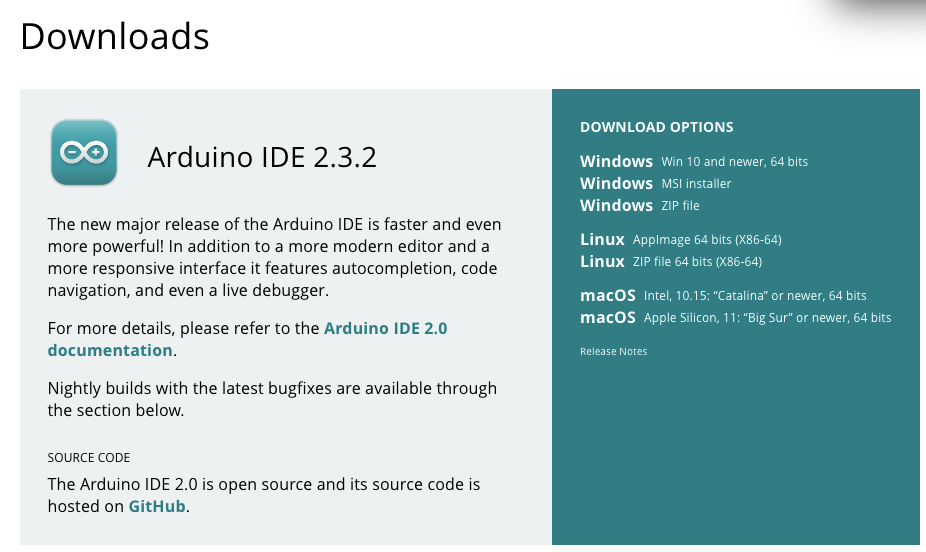
\includegraphics[width=0.5\textwidth]{anexos/instalacionArduino}
	\caption{Instalación de Arduino IDE}
	\label{fig:D.1}
\end{figure}

\subsubsection{Visual Studio Code}\label{visual-studio-code}

Visual Studio Code es el IDE empleado para el desarrollo y la implementación de la página web de PrimeBot.

Se puede obtener desde el siguiente enlace: \href{https://code.visualstudio.com/download}{Visual Studio Code}

\begin{figure}[h]
	\centering
	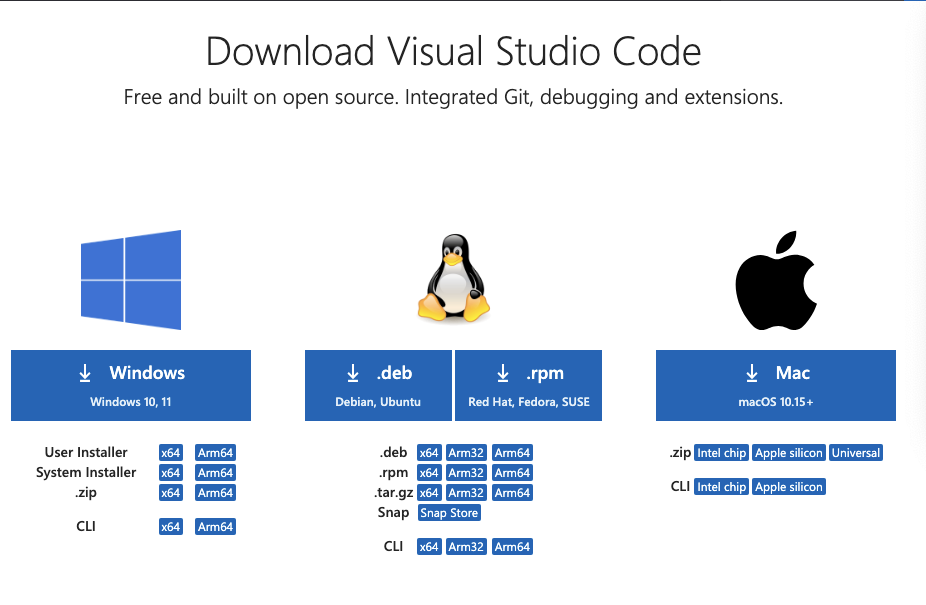
\includegraphics[width=1\textwidth]{anexos/instalacionVSCode}
	\caption{Instalación de Visual Studio Code}
	\label{fig:D.2}
\end{figure}

\subsubsection{git}\label{git}

Para hacer uso del repositorio se necesita tener instalado el gestor de versiones Git. Este programa permite clonar el repositorio, movernos dentro de el... etc.

Se puede obtener desde: \href{https://www.git-scm.com/downloads}{GIT}

Cuando esté instalado, trabajaremos con Git Bash.

\begin{figure}[h]
	\centering
	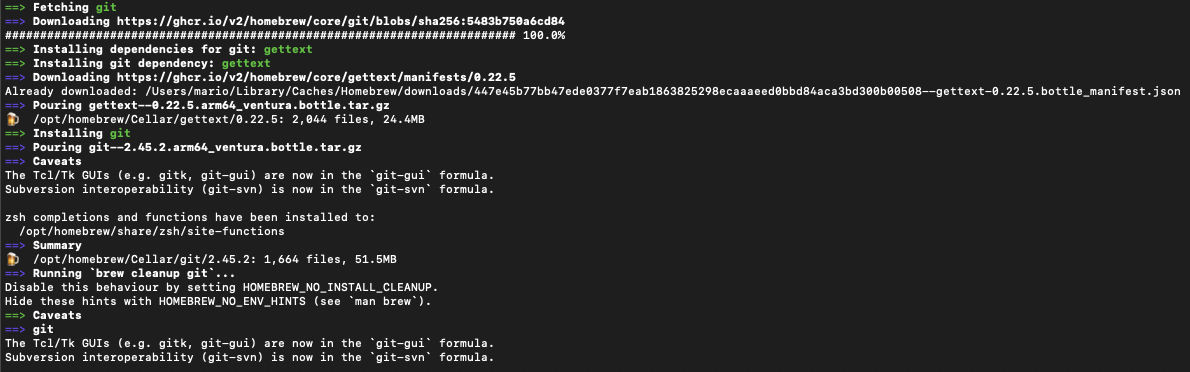
\includegraphics[width=1\textwidth]{anexos/instalacionGit}
	\caption{Instalación de Git}
	\label{fig:D.3}
\end{figure}

\subsection{Obtención del código fuente}\label{obtencion-del-codigo-fuente}

Para el desarrollo de los algoritmos empleados en PrimeBot se ha utilizado el repositorio Git hospedado en GitHub, lo primero es obtener una copia de la siguiente manera:
\begin{enumerate}
\def\labelenumi{\arabic{enumi}.}
\tightlist

\item
  Abrir la terminal Git Bash.
\item
  Desplazarse al directorio donde se desee copiar el repositorio
  (utilizando el comando \texttt{cd}).
  
  \item
  Introducir el siguiente comando:\\
  \texttt{git\ clone\ https://github.com/marioAlonso2122/Primebot.git}
  \item
  Se iniciará la descarga del repositorio, cuando finalice se dispondrá
  de una copia completa de este.
\end{enumerate}

\begin{figure}[h]
	\centering
	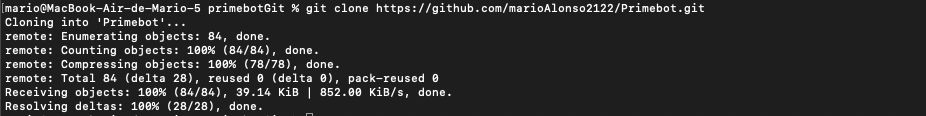
\includegraphics[width=1\textwidth]{anexos/obtenerRepositorio}
	\caption{Obtener repositorio}
	\label{fig:D.4}
\end{figure}

\subsubsection{Añadir nuevas funcionalidades}\label{nuevas-funcionalidades}

Una vez dispongamos de una copia del repositorio de PrimeBot en nuestro equipo ya podremos realizar la incorporación de nuevas funcionalidades al código de la siguiente manera:

\begin{enumerate}
\def\labelenumi{\arabic{enumi}.}
\tightlist

\item
Abrir el archivo main.ino con el editor de código Arduino.
\item
Debemos dejar las definiciones iniciales intactas ya que son los pines de las conexiones de la PCB que deben estar estáticas o PrimeBot podría dejar de funcionar.
\item
Tenemos que localizar la función llamada primeBotAction.
\item
Dentro de esta función disponemos de un recurso switch-case donde podremos incorporar nuevas funcionalidades.
\item
En el main.ino que se descargar del repositorio encontramos los 4 primeros case ya ocupados, cada valor de case corresponde a uno de los valores obtenidos a través del switch dip integrado en el PCB.
\item
Dentro del case podemos añadir nuevos valores donde incorporar nuevas funcionalidades a PrimeBot.
Se recomienda dejar un valor de case para cada funcionalidad nueva.
\item
Hay que incorporar dentro de la nueva funcionalidad un bucle while(true) que solo salga cuando se pulse el botón para poder ejecutar constantemente la funcionalidad hasta que se pulse de nuevo el botón de cambio de función.
\end{enumerate}

\begin{figure}[h]
	\centering
	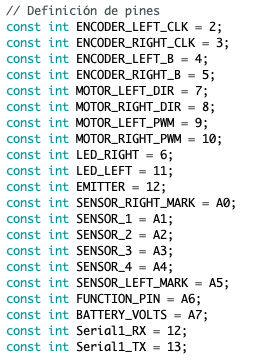
\includegraphics[width=0.5\textwidth]{anexos/definicionPines}
	\caption{Definicion de los pines de la placa en el Main}
	\label{fig:D.5}
\end{figure}

\begin{figure}[H]
	\centering
	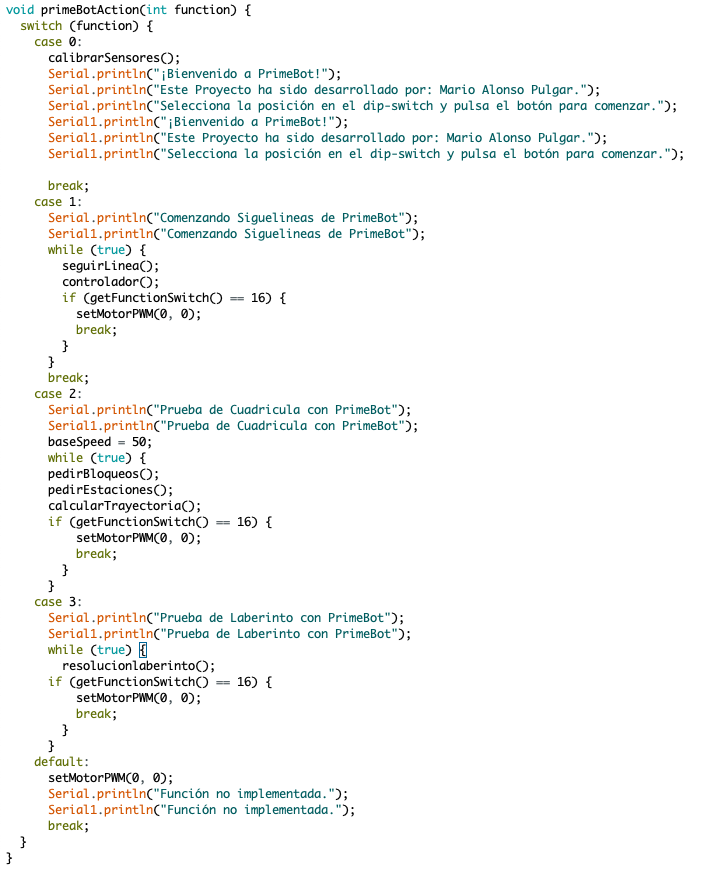
\includegraphics[width=1\textwidth]{anexos/nuevasFunciones}
	\caption{Lugar donde añadir nuevas funcionalidades}
	\label{fig:D.6}
\end{figure}


\subsubsection{Ejecutar código}\label{ejecutar-codigo}
Al estar trabajando con Arduino, el código se recomienda ejecutarlo siempre en un dispositivo real, para ello:
\begin{enumerate}
\def\labelenumi{\arabic{enumi}.}
\tightlist
\item
Conectamos la placa Arduino al equipo vía USB
\item
Dentro de las opciones del IDE de arduino en el apartado Herramientas, debemos seleccionar la placa donde vamos a cargar el código y el puerto al que está conectada esa placa.
\item
Pulsaremos en la opción subir para compilar y enviar el código a la placa arduino que vayamos a emplear.
\end{enumerate}
\begin{figure}[h]
	\centering
	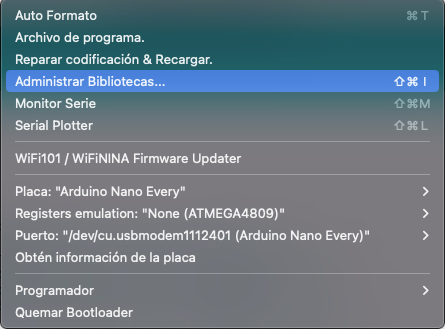
\includegraphics[width=0.5\textwidth]{anexos/seleccionarPlaca}
	\caption{Seleccion de placa en Arduino IDE}
	\label{fig:D.7}
\end{figure}

\apendice{Documentación de usuario}

\section{Introducción}

En este manual se detallan los requerimientos para utilizar todas las funcionalidades de PrimeBot y poder aprovechar cada uno de los parámetros que hay en la programación del robot.

\section{Requisitos de usuarios}

Los requisitos mínimos para poder utilizar el proyecto son:

\begin{itemize}
\tightlist
\item
  Disponer de un kit de PrimeBot con main.ino cargado
  \item
  Disponer de un móvil Android o un equipo con conexión Bluetooth
  \item
  Disponer de una aplicación como Monitor Serial
\end{itemize}

\section{Instalación}

Si el usuario ya dispone del programa main.ino cargado en la placa de Arduino correspondiente y una aplicación de monitor serial instalada en el dispositivo a conectar, no deberá realizar ninguna instalación adicional.

\section{Manual del usuario}

En esta sección se describe el uso de las diferentes funcionalidades de PrimeBot
\subsection {Conexión Bluetooth}

Antes de ejecutar cualquier programa, debemos encender PrimeBot y realizar la conexión Bluetooth.
Cuando esta conexión esté hecha, el LED rojo del módulo Bluetooth permanecerá fijo.

\subsection {Modo Calibración}

El modo calibración corresponde a la posición 0000 del dip switch que está integrado en la placa de control.

Cuando se quiere utilizar PrimeBot, este es el primer modo que debemos ejecutar ya que en este modo se realiza la calibración de los sensores siguelíneas QTR y se establece la conexión Bluetooth con el robot.
El orden correcto de ejecución será:

\begin{enumerate}
\def\labelenumi{\arabic{enumi}.}
\tightlist
\item
Seleccionamos la posición 0000 en el switch.
\item
Se pulsa el botón de selección de programa.
\item
Mientras la luz LED de la plaza arduino esté encendida de forma fija, debemos hacer pasadas suaves sobre la línea negra que debe seguir, de esta forma estaremos calibrando los sensores.
\item
Cuando acabe la calibración de los sensores, los motores se moverán durante un segundo indicando que la calibración ha terminado.
\item
Ahora podemos realizar la conexión Bluetooth con PrimeBot desde nuestro dispositivo.
\end{enumerate}

\begin{figure}[h]
	\centering
	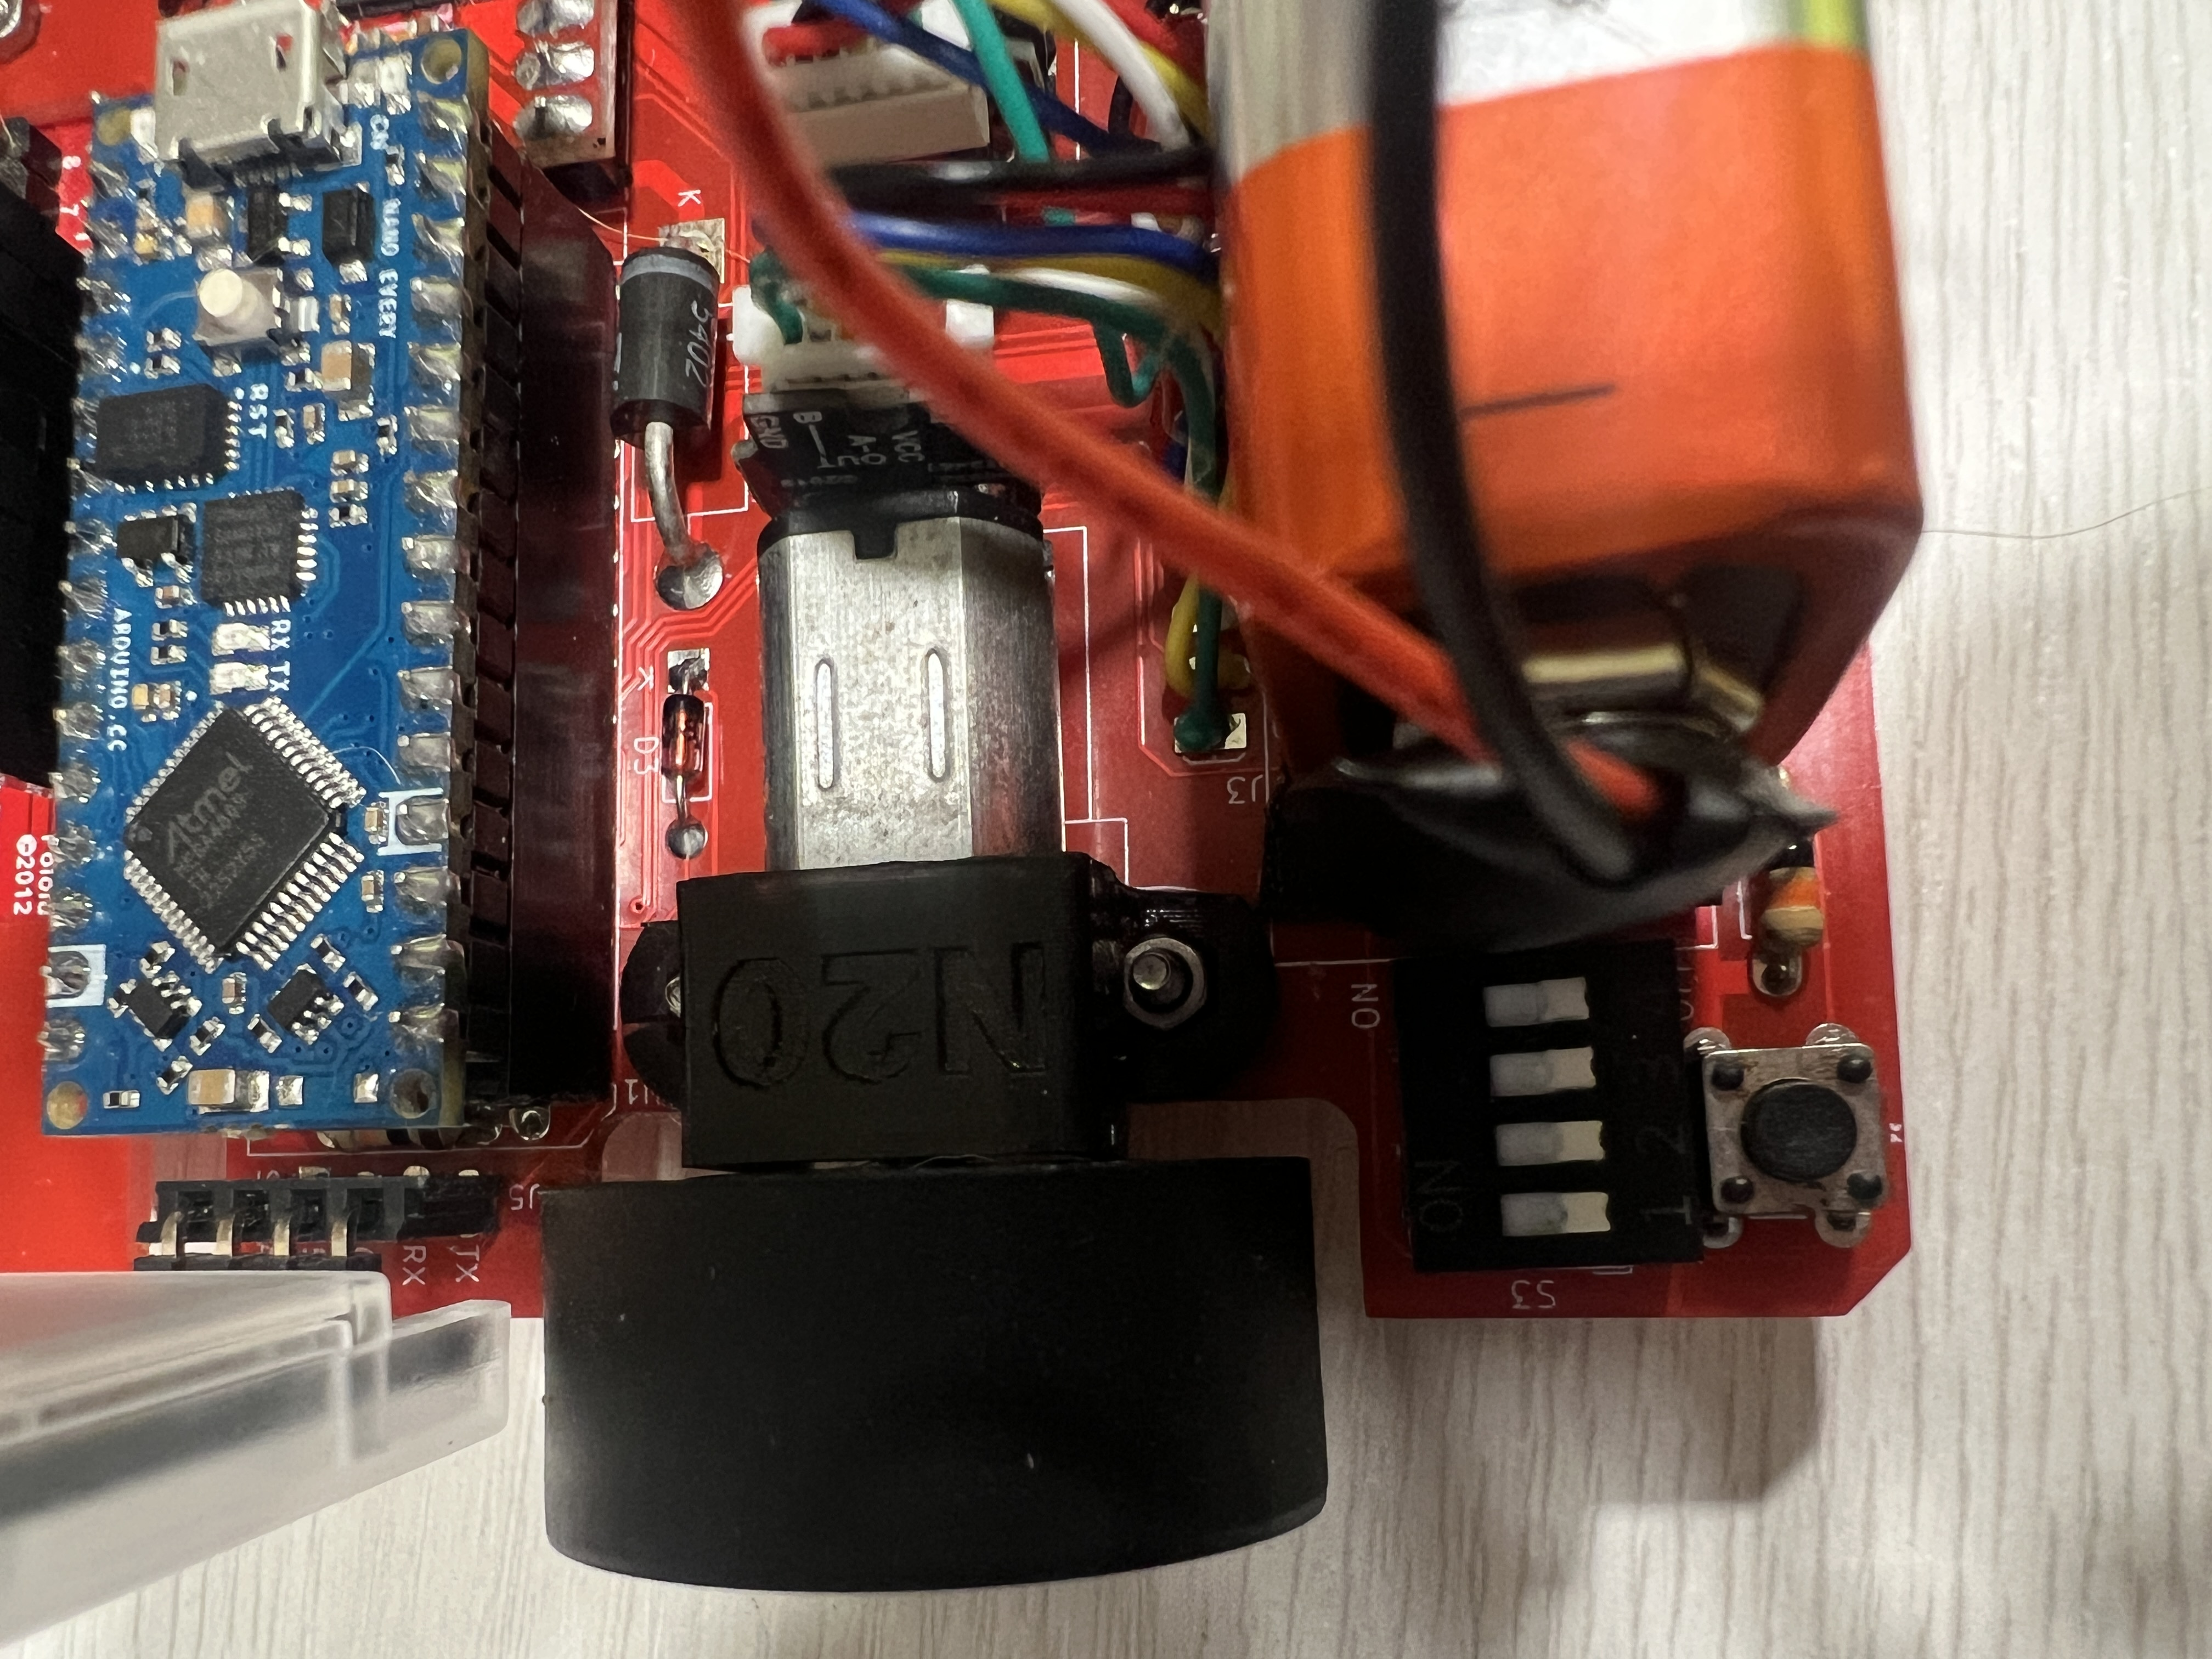
\includegraphics[width=0.5\textwidth]{anexos/0000}
	\caption{Posición Modo Calibración}
	\label{fig:E.1}
\end{figure}


\subsection {Modo Siguelíneas}
Esta funcionalidad corresponde a la posición 0001 del dip switch integrado en la placa de control.
El modo siguelíneas consiste en el seguimiento de una línea negra sobre un fondo blanco de cara a realizar las vueltas al circuito cerrado en el menor tiempo posible y con la mayor estabilidad posible del robot.

\begin{enumerate}
\def\labelenumi{\arabic{enumi}.}
\tightlist
\item
Tras realizar la calibración y la conexión por Bluetooth, colocaremos a PrimeBot sobre la línea negra a seguir.
\item
Colocaremos el switch en la posición 0001.
\item
Se pulsa el botón de selección de programa.
\item
Si hemos hecho bien los pasos en la aplicación de Monitor Serial veremos un mensaje indicando que se ejecutará el código correspondiente a la prueba siguelíneas.
\item
PrimeBot comenzará a moverse por la línea negra
\end{enumerate}

\begin{figure}[h]
	\centering
	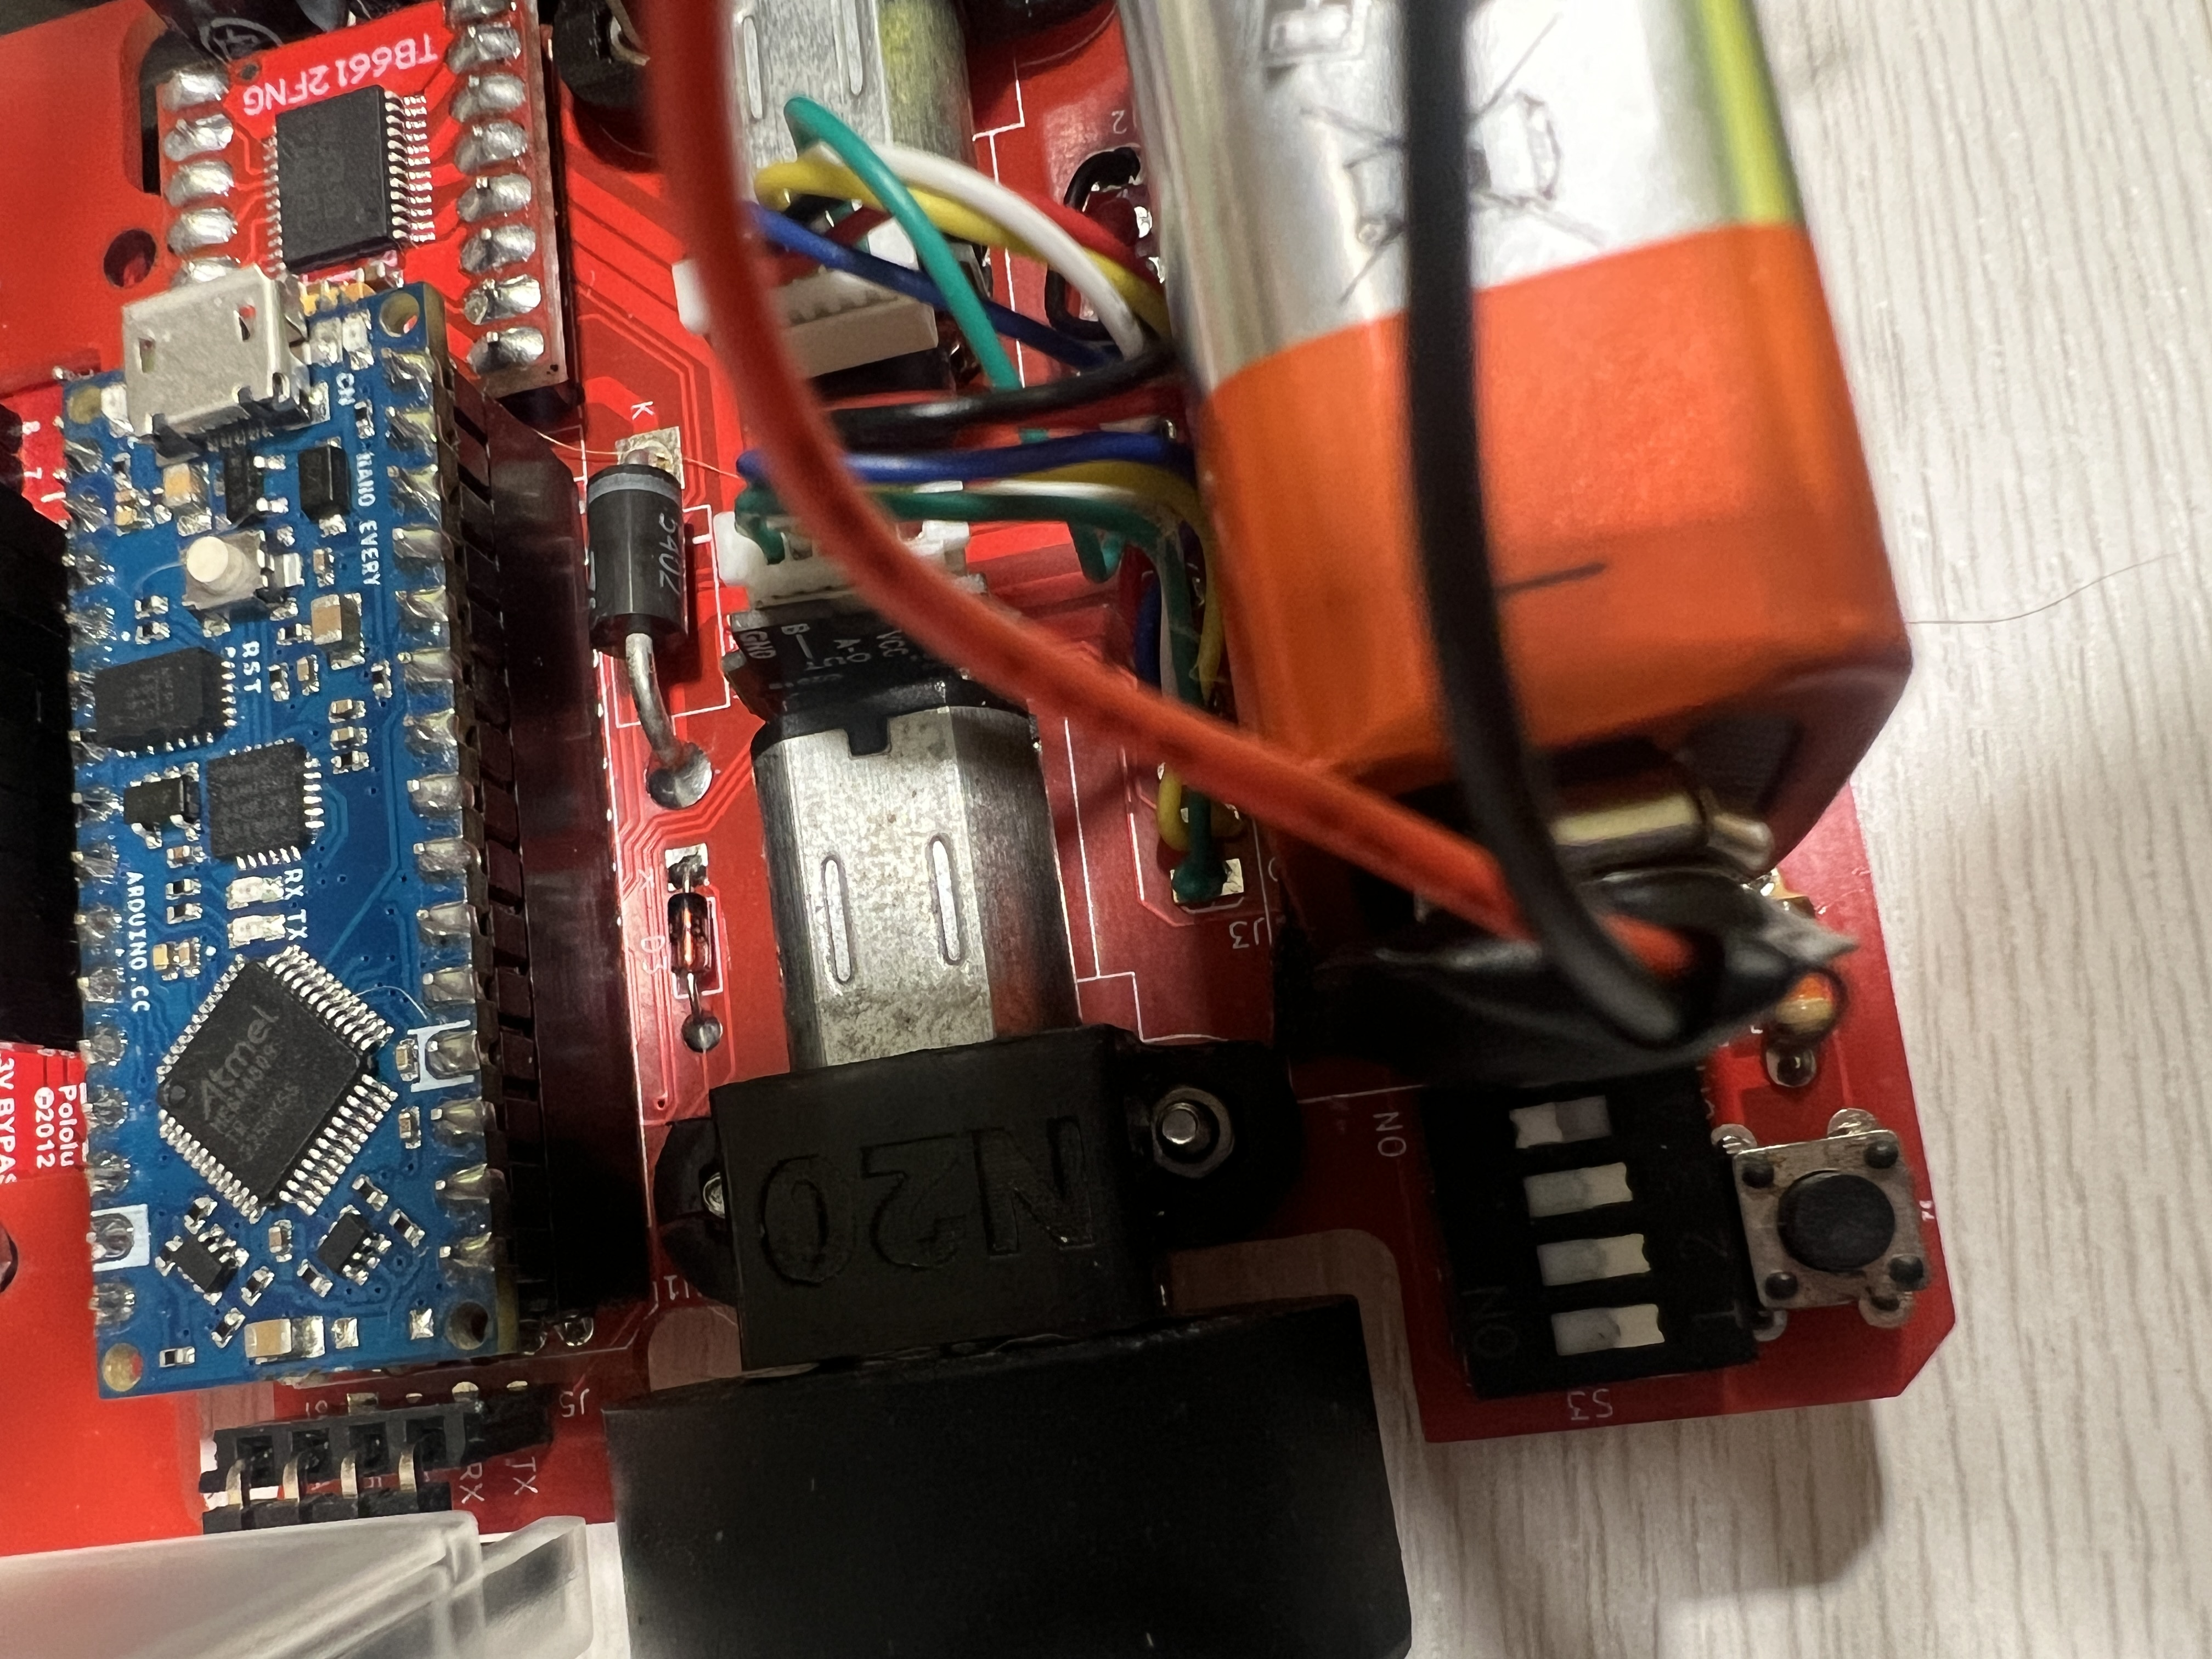
\includegraphics[width=0.5\textwidth]{anexos/0001}
	\caption{Posición Prueba Siguelíneas}
	\label{fig:E.1}
\end{figure}

A la vez que se está ejecutando este algoritmo y PrimeBot se va moviendo, en el Monitor Serial veremos impresos diferentes parámetros los cuales son configurables enviando carácteres a través de Monitor Serial de la siguiente forma:
\begin{itemize}
\tightlist
\item
  P: Aumentará la variable Kp en 0.1
  \item
  p: Reducirá la variable Kp en 0.1
  \item
  I: Aumentará la variable Ki en 0.01
   \item
  i: Reducirá la variable Ki en 0.01
   \item
  D: Aumentará la variable Kd en 0.1
   \item
  d: Reducirá la variable Kd en 0.1
   \item
  V: Aumentará la variable Kv en 0.01
   \item
  v: Reducirá la variable Kv en 0.01
   \item
  B: Aumentará la variable Velocidad base en 1
   \item
  b: Reducirá la variable Velocidad base en 1
\end{itemize}

\subsection {Modo Cuadrícula}
Esta funcionalidad corresponde a la posición 0010 del dip switch integrado en la placa de control.

El modo cuadrícula está pensado para la navegación de PrimeBot a través de una cuadrícula ya definida en dimensiones y otorgando a PrimeBot una estación de origen y una de destino.
La ejecución correcta de este programa será:

\begin{enumerate}
\def\labelenumi{\arabic{enumi}.}
\tightlist
\item
Seleccionamos la posición 0010 en el switch.
\item
Se pulsa el botón de selección de programa.
\item
Colocamos a PrimeBot en la estación de origen que corresponda.
\item
A través del monitor serial nos comunicaremos con PrimeBot.
\item
El primer parámetro que tenemos que poner es el número de puntos bloqueados, en caso de poner un valor mayor que 0, PrimeBot solicitará las coordenadas X e Y de los puntos bloqueados.
\item
Seguido nos solicitará la estación de Origen donde ya está situado PrimeBot.
\item
Por último nos solicitará la estación de destino.
\item
PrimeBot comenzará a navegar por la cuadrícula hasta llegar a la estación de destino.
\end{enumerate}

\begin{figure}[h]
	\centering
	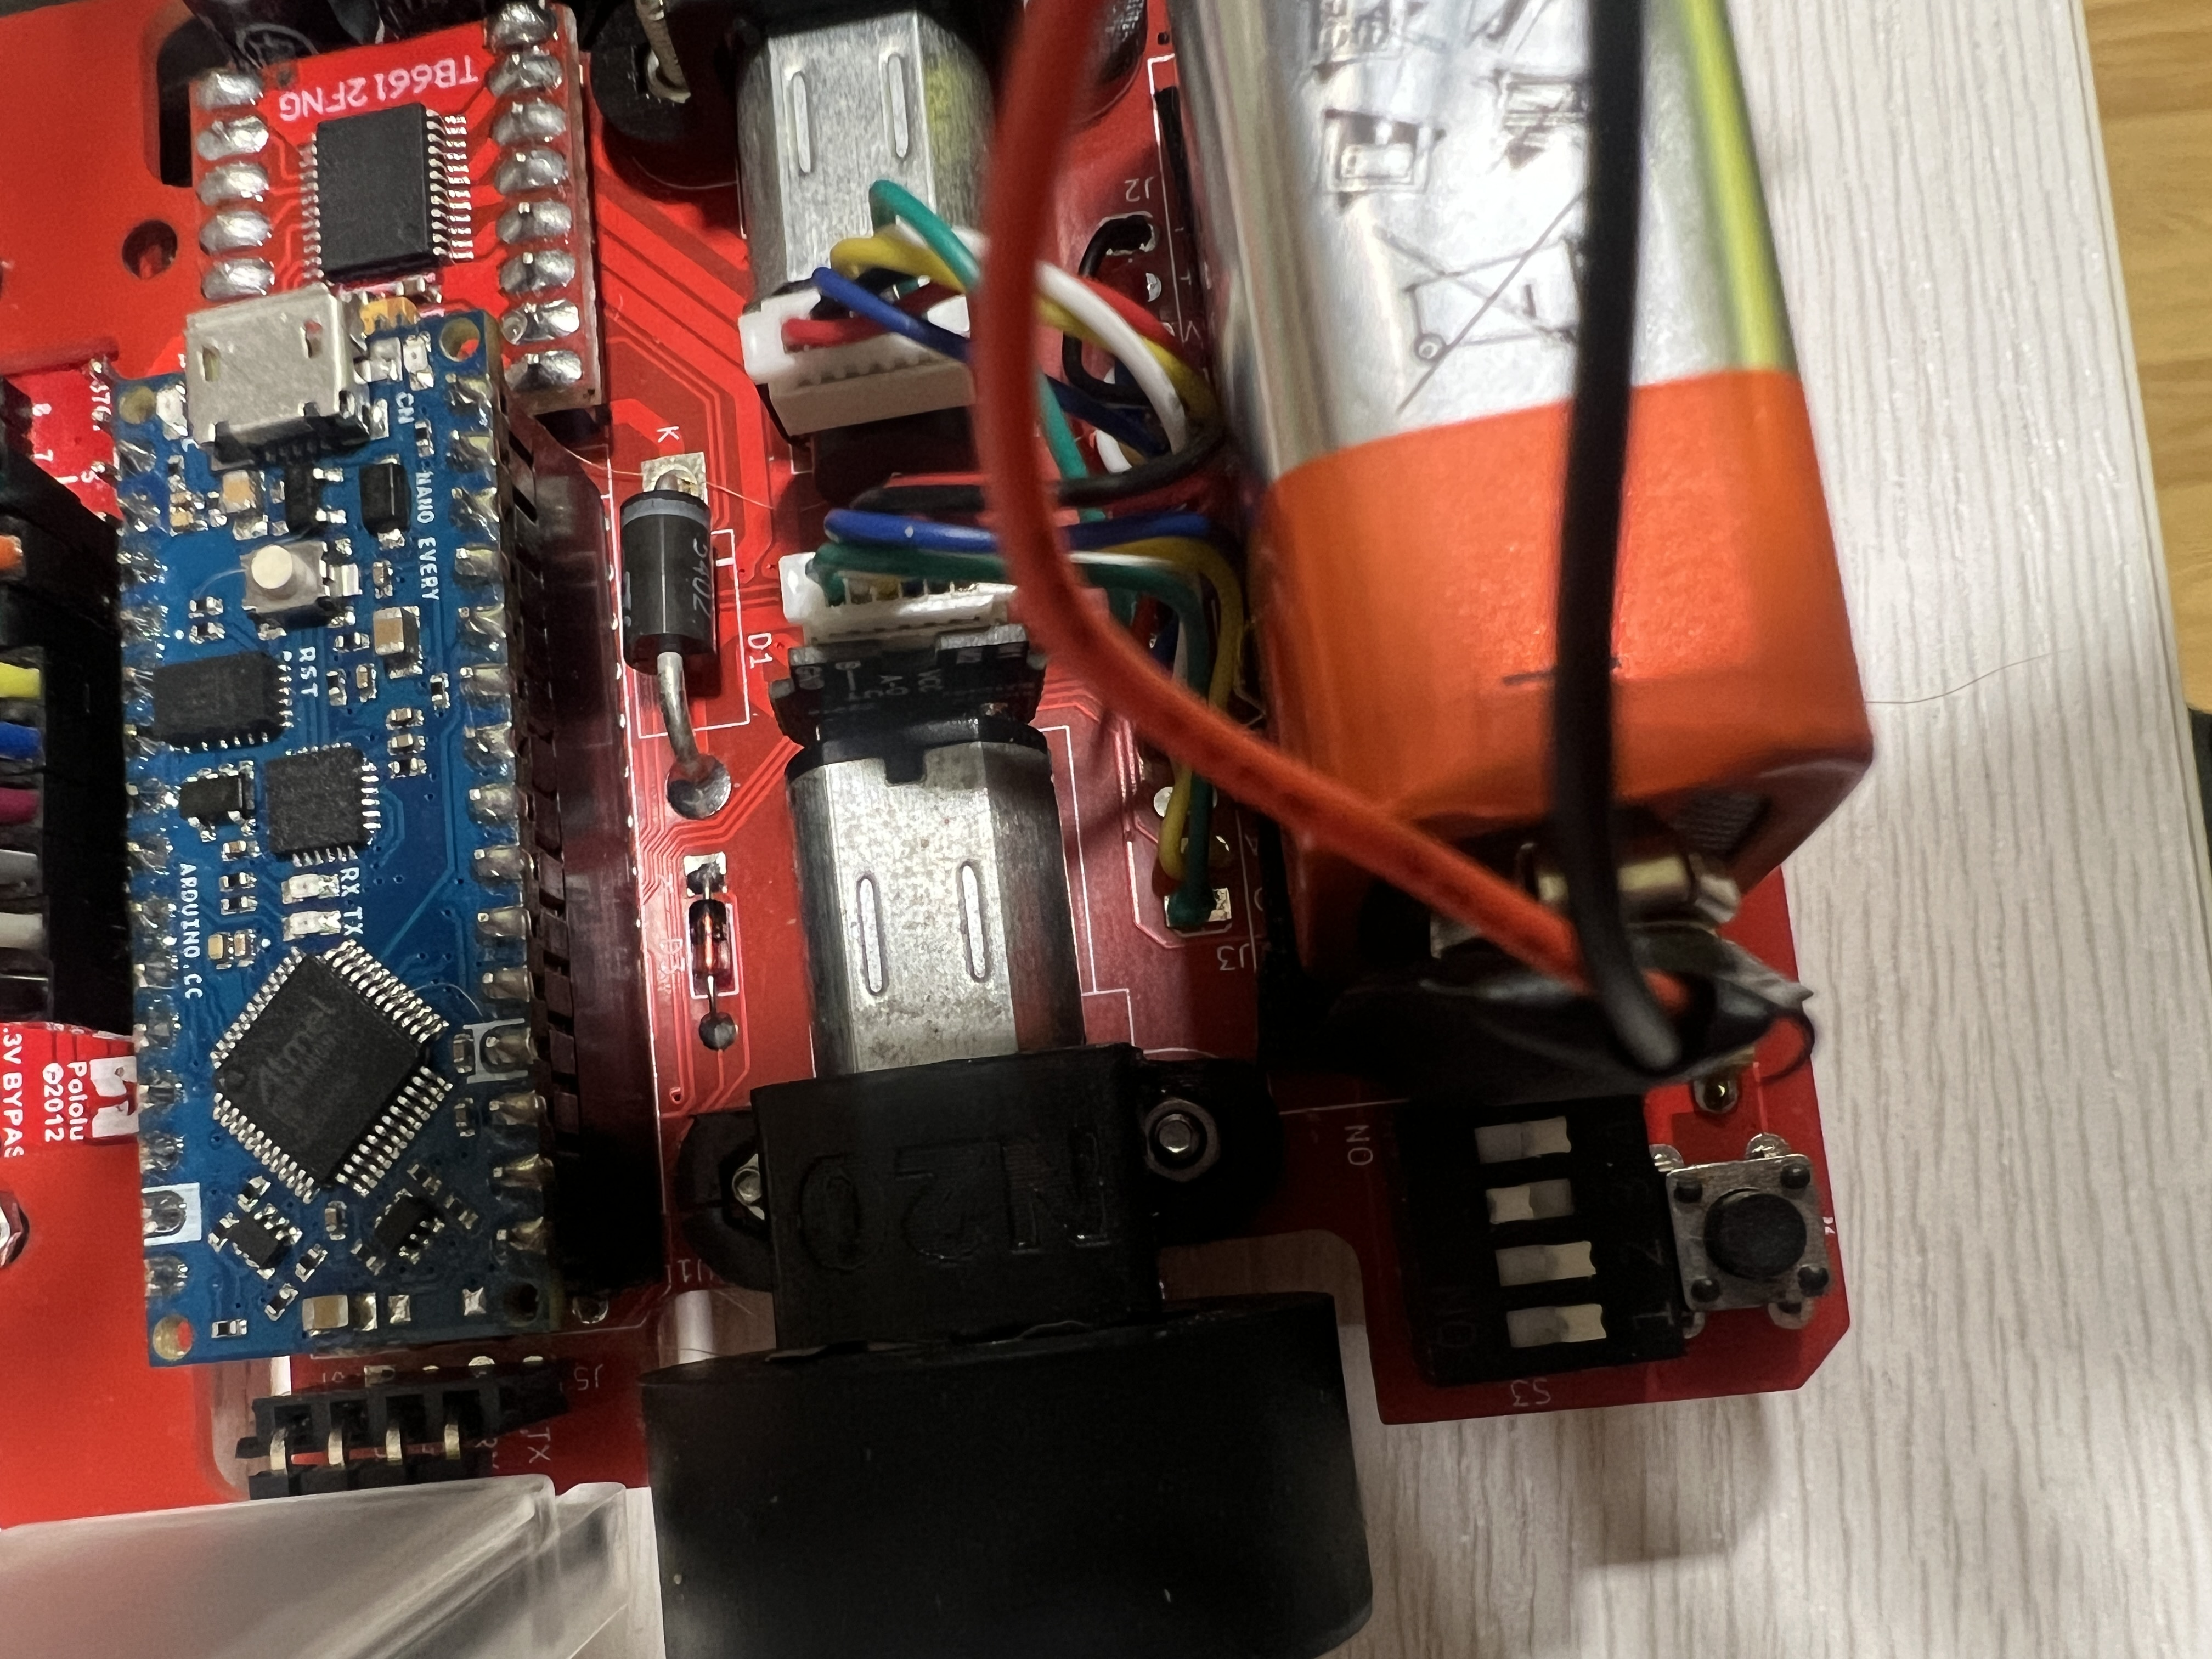
\includegraphics[width=0.5\textwidth]{anexos/0010}
	\caption{Posición Prueba Cuadrícula}
	\label{fig:E.1}
\end{figure}

En el caso de que no sea posible calcular una ruta debido a los puntos bloqueados, PrimeBot nos lo comunicará por el Monitor serial y se deberá pulsar de nuevo el botón de selección de programa.
Además, a través del monitor serial PrimeBot imprimirá una cuadrícula igual a la real indicando tanto el recorrido que está realizando como los puntos bloqueados.

Esta prueba también emplea un algoritmo PID para navegar a través de la cuadrícula por tanto podemos modificar los parámetros que hemos nombrado en el apartado anterior si lo vemos necesario.

\subsection {Modo Laberinto}
Esta funcionalidad corresponde a la posición 0011 del dip switch integrado en la placa de control.
\begin{enumerate}
\def\labelenumi{\arabic{enumi}.}
\tightlist
\item
Seleccionamos la posición 0011 en el switch.
\item
Colocamos a PrimeBot en el origen del laberinto.
\item
PrimeBot recorrerá el laberinto hasta encontrar la salida.
\end{enumerate}

\begin{figure}[h]
	\centering
	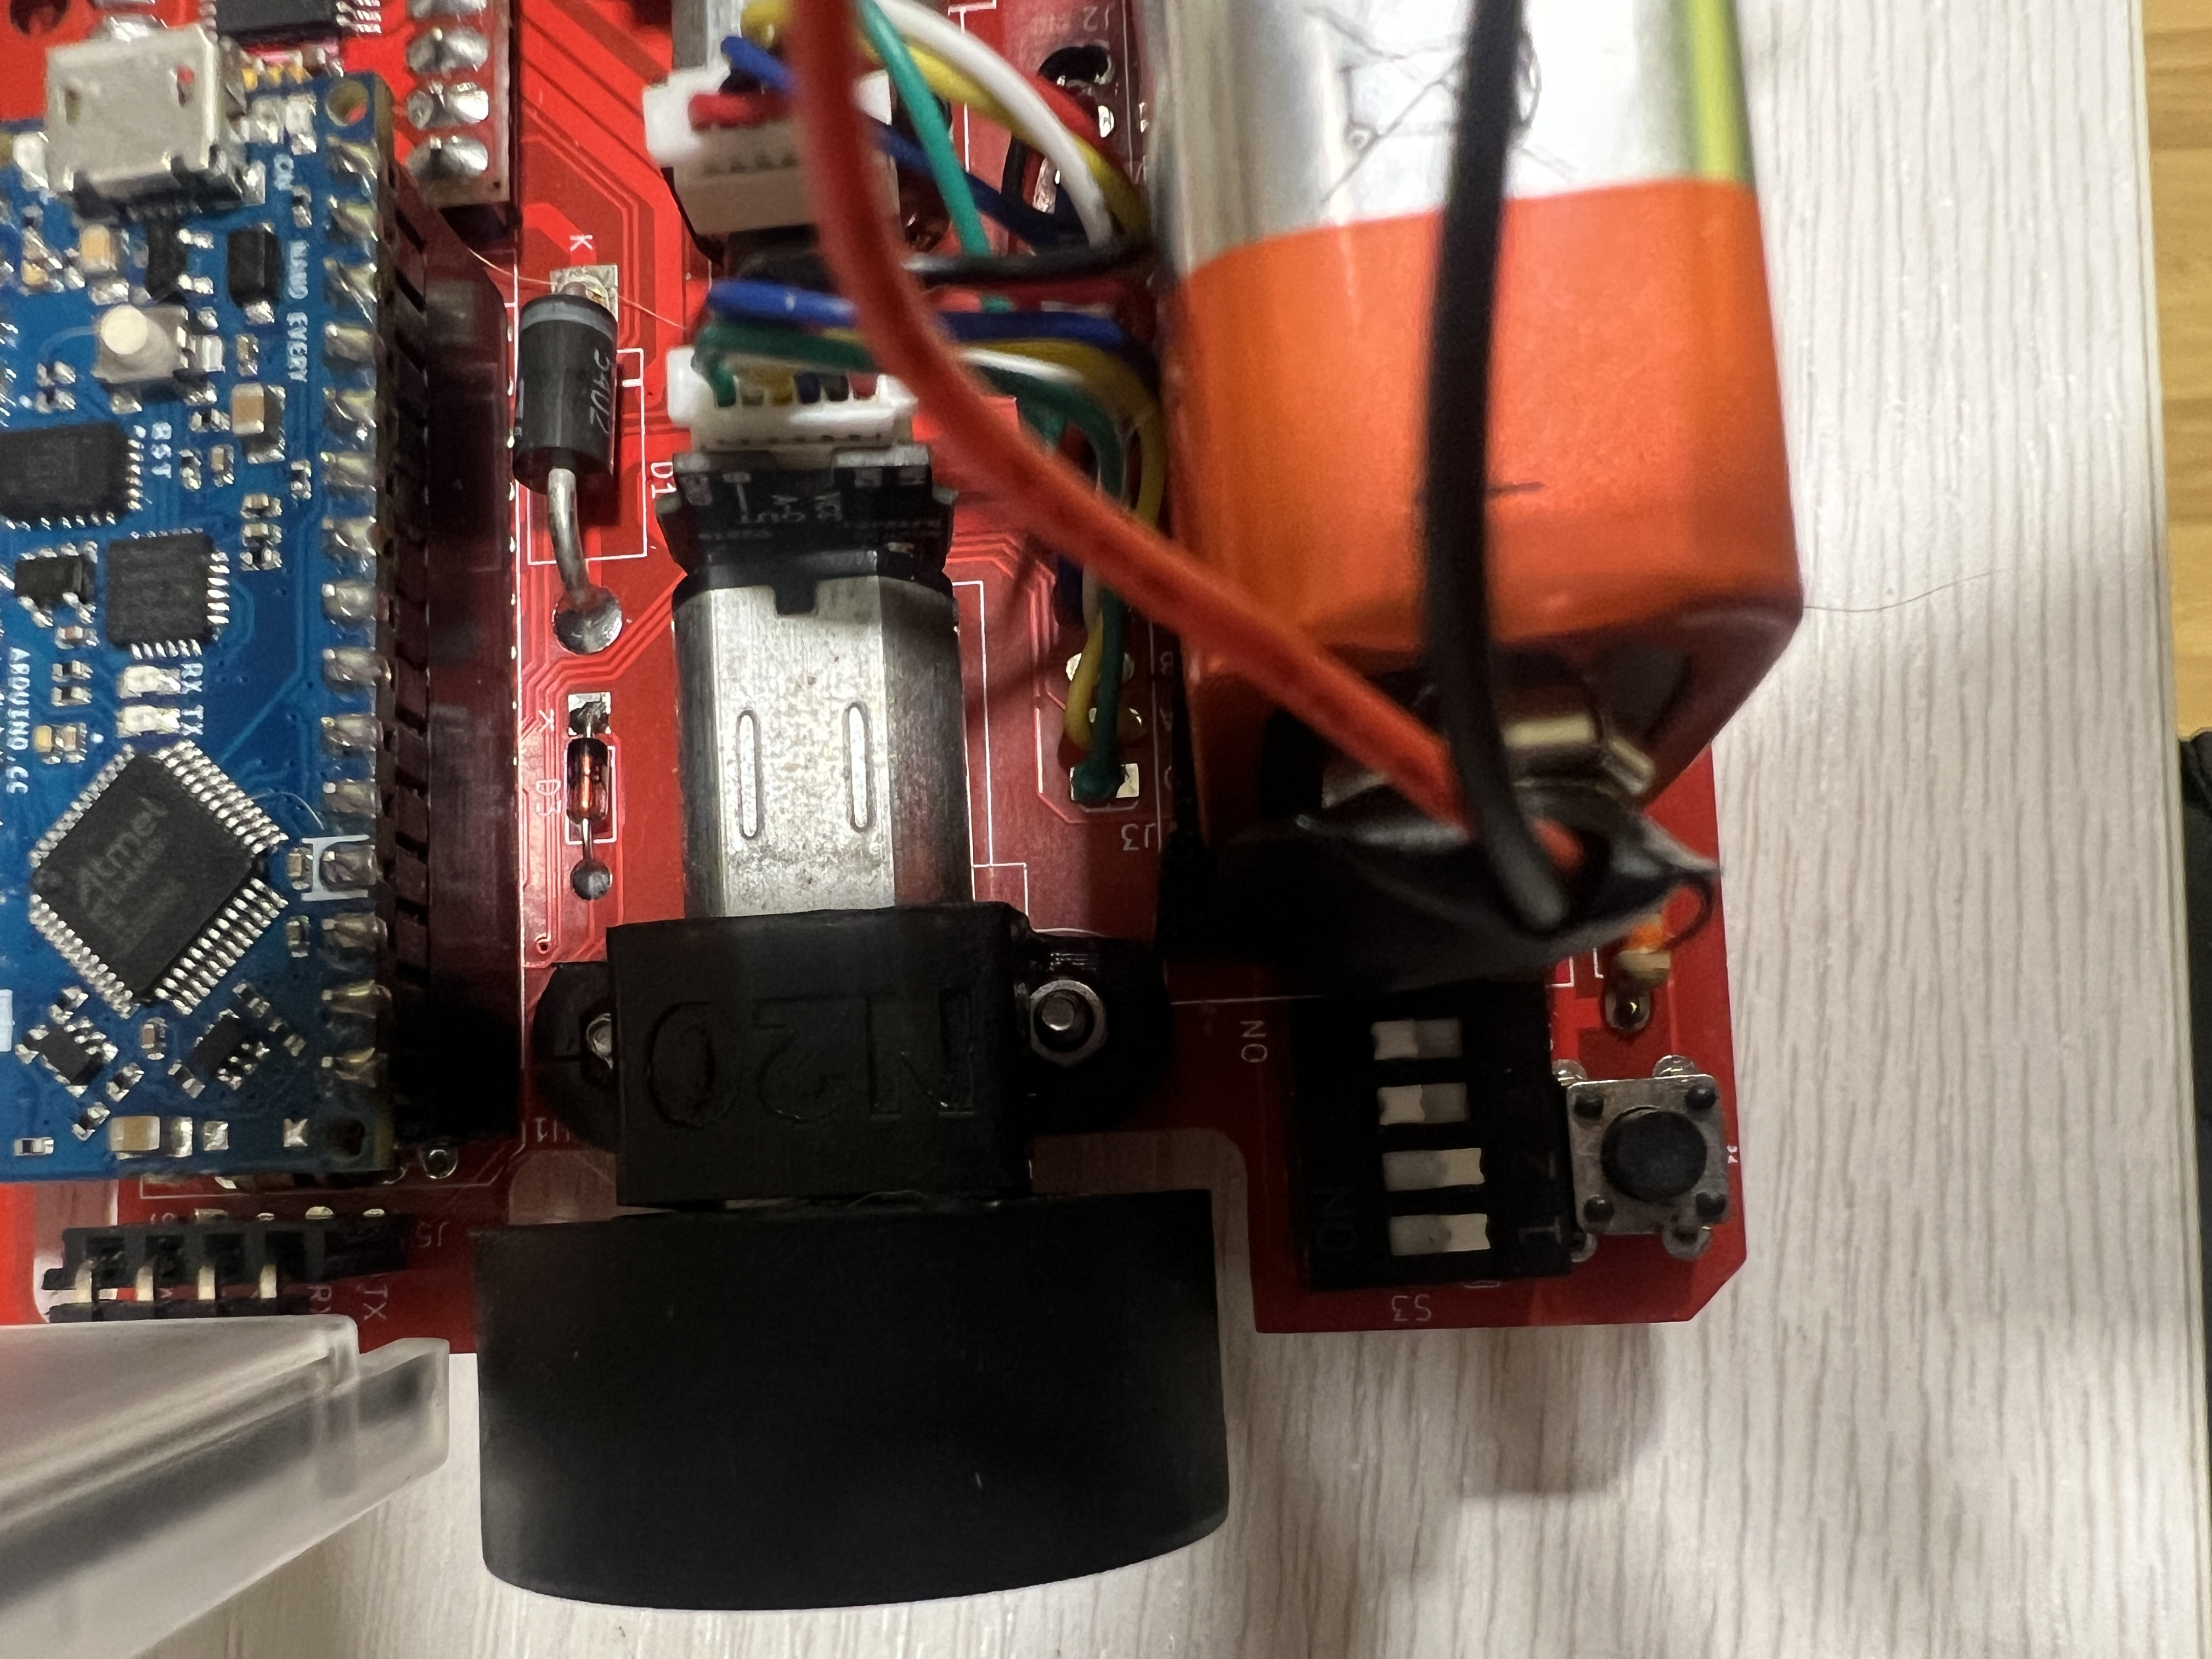
\includegraphics[width=0.5\textwidth]{anexos/0011}
	\caption{Posición Prueba Laberinto}
	\label{fig:E.1}
\end{figure}

\apendice{Anexo de sostenibilización curricular}

\section{Introducción}

El desarrollo de PrimeBot no solo se centró en la creación de un robot eficiente y competitivo, sino que también se consideraron aspectos importantes de sostenibilidad. Este anexo proporciona una reflexión personal sobre las competencias de sostenibilidad adquiridas durante el desarrollo del proyecto y cómo se han aplicado en el Trabajo de Fin de Grado. La sostenibilidad en la ingeniería es crucial para asegurar que las soluciones tecnológicas no solo sean efectivas, sino también responsables con el medio ambiente y la sociedad.

\section{Eleccion de materiales}

Durante el desarrollo de PrimeBot, una de las primeras consideraciones de sostenibilidad fue la elección de materiales y componentes. Se priorizaron componentes electrónicos de bajo consumo energético, como el Arduino Nano y los sensores de Pololu, que son eficientes y reducen el impacto ambiental. Además, se utilizó un PCB personalizado para minimizar el uso de cables y componentes adicionales, reduciendo así los residuos electrónicos.

Además los componentes realizados a través de impresión 3D han sido fabricados con los materiales menos contaminantes que hay en el mercado.

\section{Optimización energética}
El algoritmo PID y otros algoritmos de control fueron diseñados para ser eficientes en términos de consumo de energía. PrimeBot fue programado para optimizar el uso de energía de los motores y sensores, lo que no solo mejora el rendimiento del robot, sino que también extiende su vida útil y reduce la necesidad de recargas frecuentes.

\section{Reciclaje y Reutilización}

Otro aspecto de sostenibilidad abordado en el proyecto fue el reciclaje y la reutilización de componentes. Muchos de los componentes utilizados en PrimeBot fueron reutilizados de proyectos anteriores, reduciendo la necesidad de adquirir nuevos materiales. 

\section{Gestión de Residuos}
La gestión de residuos fue un aspecto clave en todas las fases del proyecto. Durante la fase de prototipado, se implementaron prácticas para minimizar los residuos generados, como la reducción de impresiones y el uso eficiente de materiales durante el montaje del PCB. Los componentes obsoletos o defectuosos fueron desechados de acuerdo con las normativas de gestión de residuos electrónicos.

\section{Conclusión}
El desarrollo de PrimeBot me permitió adquirir y aplicar diversas competencias de sostenibilidad, desde el uso responsable de recursos y la optimización energética, hasta la promoción de la economía circular y la educación social. Estas competencias no solo son relevantes para el proyecto específico de PrimeBot, sino que también serán esenciales en mi futura carrera como ingeniero. La integración de prácticas sostenibles en proyectos de ingeniería es crucial para contribuir a un futuro más sostenible y responsable.


\bibliographystyle{plain}
\bibliography{bibliografiaAnexos}

\end{document}
